\documentclass[lettersize,journal]{IEEEtran}
\usepackage{amsmath,amsfonts}
\usepackage{algorithmic}
\usepackage{algorithm}
\usepackage{array}
\usepackage[caption=false,font=normalsize,labelfont=sf,textfont=sf]{subfig}
\usepackage{textcomp}
\usepackage{stfloats}
\usepackage{url}
\usepackage{verbatim}
\usepackage{graphicx}
\usepackage{xcolor}
\usepackage{csquotes}
\usepackage{makecell}
% my added packages and commands =======================
\usepackage[numbers]{natbib} %removed cite package
\usepackage{tikz}
\usetikzlibrary{positioning,shapes.geometric}
\usepackage{adjustbox}
\usepackage{listings}
\usepackage{caption}         
\captionsetup[lstlisting]{justification=centering, singlelinecheck=false}
\providecommand{\gls}[1]{#1}
\definecolor{highlight}{RGB}{00,150,00}
\definecolor{todo}{RGB}{200,50,00}
\definecolor{rank1}{HTML}{70FF70}
\definecolor{rank2}{HTML}{858585}
\definecolor{rank3}{HTML}{454545}
\definecolor{rank4}{HTML}{000000}
\newcommand{\SIMSESpec}{\texttt{SIMSE\_Spec}}
\newcommand{\LoneSpec}{\texttt{L1\_Spec}}
\newcommand{\JTFS}{\texttt{JTFS}}
\newcommand{\DTWEnv}{\texttt{DTW\_Envelope}}
\newcommand{\LossSelect}{\textbf{Loss Selection}}
\newcommand{\SynthSelect}{\textbf{Synthesis Selection}}
\newcommand{\PeriodicLoss}{\textbf{Periodic Loss}}
\newcommand{\OutDomain}{\textbf{Out-Domain Generation}}
\newcommand{\BPNoise}{\textbf{BP-Noise}}  
\newcommand{\AddSineSaw}{\textbf{Add-SineSaw}}  
\newcommand{\AmpMod}{\textbf{Noise-AM}}  
\newcommand{\FMMod}{\textbf{SineSaw-AM}}  

% code_style.tex
\usepackage{xcolor}
\usepackage{tikz}

\newcommand{\greencircle}{%
    
\begin{tikzpicture}
        \fill[green] (0,0) circle (4pt); % Adjust the size here if needed
    \end{tikzpicture}%
}

\newcommand{\greenstar}{%
    
\begin{tikzpicture}[scale=0.22]
        \fill[green] 
            (0,1) 
            -- (0.2245,0.309) 
            -- (1,0.309) 
            -- (0.3633,-0.118) 
            -- (0.5878,-0.809) 
            -- (0,-0.382) 
            -- (-0.5878,-0.809) 
            -- (-0.3633,-0.118) 
            -- (-1,0.309) 
            -- (-0.2245,0.309) 
            -- cycle;
    \end{tikzpicture}%
}

\newcommand{\redcircles}{
    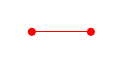
\begin{tikzpicture}[scale=0.75, line cap=round, line join=round]
        % Define coordinates for circles
        \coordinate (A) at (0,0);
        \coordinate (B) at (1,0);
        \coordinate (C) at (2,0);
        \coordinate (D) at (3,0);
        
        % Draw circles
        \foreach \point in {A,B} 
            \fill[red] (\point) circle (2pt);
        
        % Connect circles with lines
        \draw[red] (A) -- (B);
    \end{tikzpicture}%
}

\lstdefinelanguage{Faust}{
    morekeywords={import, process, environment, declare, with, if, else, while, for, int, float, true, false},
    sensitive=true,
    morecomment=[l]{//}, % Line comment
    morecomment=[s]{/*}{*/}, % Block comment
    morestring=[b]", % Strings
}

% Customize the appearance of the code
\lstset{
    language=Faust,
    backgroundcolor=\color{lightgray!20},
    basicstyle=\ttfamily\small,
    keywordstyle=\color{blue}\bfseries,
    stringstyle=\color{orange},
    commentstyle=\color{green}\itshape,
    showstringspaces=false,
    numbers=left,
    numberstyle=\tiny,
    frame=single,
    breaklines=true
}

% Suppress the "Listing #" label and caption text
% \captionsetup[lstlisting]{
%     labelformat=empty,
%     labelsep=none,
%     font=normalfont,
%     skip=0pt
% }


%  ================================
\begin{document}
\title{Evaluating Sound Similarity Metrics for Differentiable, Iterative Sound-Matching}

\author{Amir Salimi, Abram Hindle, Osmar R. Za{\"i}ane}

\markboth{IEEE TRANSACTIONS ON AUDIO, SPEECH AND LANGUAGE PROCESSING, VOL -, 2025}%
{Shell \MakeLowercase{\textit{et al.}}: A Sample Article Using IEEEtran.cls for IEEE Journals}

\maketitle

\begin{abstract}
Manual sound design with a synthesizer is inherently iterative: an artist compares the synthesized output to a mental target, adjusts parameters, and repeats until satisfied. Iterative sound-matching automates this workflow by continually programming a synthesizer under the guidance of a loss function (or similarity measure) towards a target sound. Prior comparisons of loss functions have typically favored one metric over another, but only within narrow settings: limited synthesis methods, few loss types, often without blind listening tests. This leaves open the question of whether a universally optimal loss exists, or the choice of loss remains a creative decision conditioned on the synthesis method and the sound designer's preference. We propose differentiable iterative sound-matching as the natural extension of the available literature, since it combines the manual approach to sound design with modern advances in machine learning. To analyze the variability of loss function performance across synthesizers, we implemented a mix of four novel and established differentiable loss functions, and paired them with differentiable subtractive, additive, and AM synthesizers. For each of the sixteen synthesizer–loss combinations, we ran 300 randomized sound-matching trials. Performance was measured using parameter differences, spectrogram-distance metrics, and manually assigned listening scores. We observed a moderate level of consistency among the three performance measures. Our post-hoc analysis shows that the loss function performance is highly dependent on the synthesizer. These findings underscore the value of expanding the scope of sound-matching experiments, and developing new similarity metrics tailored to specific synthesis techniques, rather than pursuing one-size-fits-all solutions.
\end{abstract}

% the automatic performance measures have not been compared to human hearing
% lack of creativity in loss function definitions 
\begin{IEEEkeywords}
Audio synthesis, differentiable digital signal processing, music information retrieval, sound-matching
\end{IEEEkeywords}

\section{Introduction}
\subsection{Digital Synthesis With Sound-Matching}
Since the 1970s, artists such as Suzanne Ciani~\cite{ciani_life_in_waves} have explored the use of audio synthesizers to replicate natural sounds—such as a bottle cap popping off—in ways that preserve the essential qualities of the original while showcasing the unique characteristics of the synthesizer. Rather than merely replicating sounds, this approach uses synthesizers for artistic reinterpretation. However, the automation of this interpretive approach to sound design using digital audio synthesizers has rarely been explored, and significant knowledge gaps remain even in the simpler problem of replicating sounds. One such gap is the lack of diversity and depth in the analysis of sound-similarity measures and their interaction with various synthesis methods. As a stepping stone toward automated interpretive sound design, we use automatic and manual sound-evaluations to investigate whether the optimal choice of a sound-similarity measure is dependent on the synthesis method.

A digital audio synthesizer is any software used for the creation and manipulation of audio. Since the advent of digital signal processing (\gls{DSP}) in the 1960s~\cite{stranneby2004digital}, a wide variety of parametric audio generation functions have been proposed~\cite{lyons1997understanding,russ1999sound,shier2020spiegelib}. Manual sound design with a synthesizer is an iterative process of trial and error; when the artist has a desired (or target) sound in mind, sound design involves listening to the output, determining whether the output is closer or farther from the target, and adjusting the parameters of the synthesizer accordingly until the target is reached~\cite{russ1999sound}. This paper explores the automation of this process, which we call \textit{iterative sound-matching}. 

Automatic sound design has been a subject of research for decades, with reduction of tinkering time and creation of ``interesting" sounds as the main motivators \cite{krekovic2019insights,turian2020sorry,horner1993machine,salimi2020make,esling2019flow,engel2020ddsp,mitchell2007evolutionary,shier2020spiegelib,masuda2021soundmatch,masuda2023improving}. \textit{Sound-matching} is a common form of automatic sound design explored in literature, where a similarity metric (or loss function) is given, and the goal is to find parameters for a synthesizer that replicate \textit{all} or \textit{some} of the characteristics of a target sound as best as possible~\cite{horner1993machine,mitchell2007evolutionary,masuda2023improving}. Our analysis of past works shows that this general goal of ``sound-matching'' can be broken down in to very different subtypes, many of them rarely or never explored, despite their relevance to practical applications. This leads us to a typology of sound-matching tasks, and the importance of \textit{differentiable, iterative sound-matching}, rarely explored in previous literature~\cite{vahidi2023mesostructures}.

\textit{Iterative sound-matching} refers to works that mimic the back-and-forth process of listening to a synthesizer's output and updating the parameters until the termination conditions are met. The two necessary components are the \textit{loss function}, which determines how close two sounds are, and the \textit{parametric synthesizer} that outputs sounds based on input parameters. In the iterative workflow, a target sound is selected, the synthesizer outputs sounds based on its parameters, and the loss function determines the proximity of the output to the target. From there, the synthesizer parameters are updated, the output and target are compared, and so on. 

Despite the early popularity of the iterative approach~\cite{justice1979analytic,horner1993machine,mitchell2007evolutionary}, recent works in sound-matching have favored supervised learning using inference models, deep neural-networks (\gls{DNNs}), and large datasets. Rather than continually interacting with the environment, these models learn from a dataset of inputs (synthesizer parameters) and outputs (corresponding sound), and predict the synthesizer parameters for new sounds~\cite{yee2018automatic,han2023perceptual,han2024learning,masuda2021soundmatch,masuda2023improving}. 

Iterative sound-matching is interesting for multiple reasons. First, it better resembles the human approach to sound-design, which requires continually interacting with the environment and making decisions according to a feedback signal~\cite{sutton2018reinforcement}. Second, the trial-and-error approach leaves a trail of parameter sets from the starting point to the end goal, which could be of use to sound designers. Third, relative to the DNN-based inference models, it provides a more tractable environment with room for creative approaches to sound-similarity definitions, and more amenable to deployment on different synthesizers as it does not require pre-training on large datasets. 

This work takes a \textit{differentiable} approach to iterative sound-matching, a natural extension of early works in iterative sound-matching combined with recent advances in Machine Learning (\gls{ML}) software~\cite{braun2024dac,paszke2019pytorch} and increase in computational power~\cite{moore2012introduction,schaller1997moore}. A differentiable approach requires differentiable loss and synthesizer functions, allowing the synthesizer parameters to be updated using gradient descent~\cite{goodfellow2016deep,boyd2004convex}.

We discuss the history of sound-matching, and provide a nomenclature for different subtypes of sound-matching tasks. A number of weaknesses in current literature (see Section~\ref{sec:lacking}) are identified. The experiments in this work focus on two of these core issues, referred to as \LossSelect~and \SynthSelect. The former refers to the search for an optimal loss function, lack of novel algorithms, and the---perhaps needless---focus on outperforming state of the art (\gls{SOTA}), while the latter refers to the lack of diversity in synthesis methods.

In the case of \LossSelect, there have been many works and experiments comparing the accuracy of loss functions and choosing the best performers~\cite{vahidi2023mesostructures,turian2020sorry,engel2020ddsp,uzrad2024diffmoog,han2023perceptual,masuda2021soundmatch,turian2020sorry,bruford2024synthesizer}. We note that these claims regarding the effectiveness of one function versus another have consistently been made in limited contexts that may not generalize to other settings. One such limitation is the synthesizers used, and ties into the problem of \SynthSelect, as typically only a single (and often, simple) synthesizer has been used for testing the effectiveness of loss functions. Furthermore, there is a lack of diversity in the underlying functions used by the synthesizers, with simple Frequency Modulation (\gls{FM}) being the most common method of synthesis~\cite{horner1993machine,vahidi2023mesostructures,mitchell2007evolutionary,caspe2023envelope}. 

Considering the interplay between the two problems, we design experiments that address them simultaneously. Testing the hypothesis that the performance of a similarity measure (or loss function) is influenced by other factors in the environment, particularly the method of synthesis. We combine 4 loss functions with 4 differentiable synthesizers, and compare their performance as measured by the similarity of the final output to the target. We evaluate the final similarity with two different automatic methods, as well as manual listening tests conducted by two of the authors. We compare the distributions of the evaluation scores in order to rank the loss functions from best to worst. The results of these experiments show that when accounting for different synthesizers, there is no consistent choice of sound similarity measure for optimal performance in sound-matching.

We note that for some synthesizers, our novel use of ``dynamic time warping of envelopes'' as a loss function for differentiable sound-matching outperforms the standard methods of audio comparison. These results imply that rather than aiming to outperform the SOTA and finding a universal best performer, more effort could be placed towards diversifying the existing similarity measures of sound as well as conducting experiments using a variety of synthesis methods. Sound design is an inherently creative endeavor, and would likely benefit from a diversified range of solutions for different approaches. 

\section{Background}
\label{sec:background}
In this Section, we give a formal definition of sound-matching and the necessary components. These discussions lead to a nomenclature for types of sound-matching, as well as major perennial issues in the field. 

\subsection{Digital Audio Synthesis}
\label{sec:diffSynth}
A digital audio synthesizer is any software used for the creation and manipulation of digital audio. Digital synthesizers use signal processing chains with a variety of digital signal processing (\gls{DSP}) functions to create sounds. These functions are often parametric, and the set of parameters given to the synthesizer's chain of DSP functions is called a synthesizer program.

The simplest form of DSP function is a sinusoidal tone. For example, consider:
\[ x(n) = sin( 2\pi n T)\]

where $T$ represents time in seconds, and $n$ is the frequency parameter. If $n$ is 1, then $x(n)$ would be a waveform with a frequency of 1 hertz, meaning that the value of $x(n)$ oscillates to the same point once every second. Waveform generators are called oscillators for this reason. 

% If $n$ is in the range of 30 to 20,000 (the upper limit is often lower for some), $x(n)$ could be played as an audible tone~\cite{smith2007mathematics,jilek2014reference}.

Since the advent of digital signal processing in the 1960s~\cite{stranneby2004digital}, a wide variety of parametric audio generation functions have been proposed~\cite{lyons1997understanding,russ1999sound,shier2020spiegelib}. This includes oscillators, filters, equalizers, and envelopes, which can be used sequentially or in parallel~\cite{lyons1997understanding,russ1999sound}. Sound design with a synthesizer is done by modifying the parameters of the functions until reaching a desired output~\cite{roads1996computer,pinch2004analog}.

A relatively small subset of these synthesis methods have been used for automatic sound-matching, notably additive and/or subtractive synthesizers~\cite{esling2019flow,yee2018automatic,mitchell2007evolutionary,salimi2020make}, physical modeling~\cite{riionheimo2003parameter}, and frequency/amplitude modulation (\gls{FM}/\gls{AM})~\cite{horner1993machine,vahidi2023mesostructures}. 

Differential DSP (\gls{DDSP}) is a general term for applications that combine machine learning techniques such as gradient descent~\cite{goodfellow2016deep,boyd2004convex} with DSP~\cite{engel2020ddsp}. Implementing complex DSP functions in a differentiable manner can be challenging, and effective differentiable audio similarity measures require careful mathematical expression of the desired attributes of sound. These issues have likely contributed to the limited exploration of this domain. Perhaps to most relevant recent work is by Vahidi \textit{et al.}, featuring the comparison of two differentiable loss functions with a simple FM synthesizer~\cite{vahidi2023mesostructures}. 

\subsection{Sound Representation and Loss Functions}
\label{sec:loss_funcs}
A digital sound (or an audio signal) is a series of numbers~\cite{smith1991viewpoints,smith2007mathematics}. To compare two digital sounds, the two corresponding series are passed to a function that measures their similarity. Two signals can sound identical to our ears, without having any values in common~\cite{moore2012introduction}. This necessitates the use of proxy representations (or feature extractors) when comparing sounds automatically. Similarity between the target sound and the synthesizer output is then measured by some form of subtraction and summation of the proxy representations.

In sound-matching, particularly in a Deep Learning (\gls{DL}) context~\cite{goodfellow2016deep}, the similarity function can also be called a \textit{loss} function, where the emphasis is on measurement and reduction of the distance between target and output. It is important to note that there is a close relationship between the loss function $L$ and the sound representation function $\phi$. $L$ is the result of a distance measure $d$ applied to the features extracted by $\phi$. 

\[
L(\theta, t) = d\langle\phi(t),\phi(x)\rangle
\]

\noindent

A proxy representation is the output of the function \( \phi \), which can be thought of as a feature extraction function that maps the sounds \( t \) and \( x \) to their respective representations. 
The proportionality or distance metric $d$ has typically been the L1 distance~\cite{turian2020sorry,richard2025model}, calculated as the mean of the absolute difference between every point in the proxy representation~\cite{engel2020ddsp,vahidi2023mesostructures}:
\[
L(\theta, t) = \left\| \phi(t) - \phi(x) \right\|_1
\]

Here we discuss four methods of audio representation and the corresponding loss functions. Three of which have been used in previous works, and a novel method not previously used in iterative sound-matching. 

\subsubsection{Parameter Loss}
A common measure of similarity in sound-matching is the distance between synthesizer parameter sets, referred to as ``P-Loss"~\cite{han2023perceptual}. Typically, for the implementation of P-Loss the parameter sets are treated as vectors in space, and L1 or L2 distance is applied. There are two major limitations to this approach: First, the target and output sound must be made by the same synthesizer; otherwise the parameter sets cannot be compared (see Section~\ref{sec:matching_types}). Second, the relationship between synthesizer parameters and the audio output is not linear~\cite{shier2020spiegelib,han2023perceptual,esling2019flow}. 

\subsubsection{Fourier Spectrograms}
\label{sec:fourier_specs}
Fourier-based transformations such as short-time Fourier transforms (\gls{STFT}), Mel-spectrograms, and Mel-frequency cepstral coefficients have been viewed as the de facto and state-of-the-art representation of audio~\cite{beauchamp2003error,mitchell2007evolutionary,yee2018automatic}, however, there are many issues associated with their use in sound-matching~\cite{turian2020sorry,vahidi2023mesostructures,han2023perceptual,uzrad2024diffmoog}. Fourier transformations allow for the conversion of a signal from the time-domain to the frequency domain. Audio spectrograms can be generated by segmentation of a piece of audio into overlapping windows followed by the application of Fourier transforms to each window. They are costly to compute, but provide a better temporal view of changes in frequency content~\cite{muller2007dynamic,smith2007mathematics}. There are different types of spectrograms that have a basis in Fourier transformations, but the most notable and commonly used is the STFT.  

What we call \textit{Fourier-based Spectrograms} are variations on the STFT approach. For example, Mel-Spectrograms \textit{bin} frequencies on a near-logarithmic scale to better match human perception of frequencies~\cite{muller2007dynamic}. Multi-scale spectrograms (\gls{MSS}) used in recent works are a simple weighted average of multiple spectrograms with different parameters such as window size, number of frequency bins, and hop size~\cite{engel2020ddsp,vahidi2023mesostructures}; this may provide some improvements at a higher computational cost~\cite{turian2020sorry,engel2020ddsp}.


\subsubsection{Joint-Time Frequency Spectrum}
Recent works have focused on the limitations of parameter and spectral loss functions in sound-matching~\cite{vahidi2023mesostructures,uzrad2024diffmoog}, seeking to create more effective general solutions for the comparison of audio. 
Noting the aforementioned weaknesses of comparing STFT spectrograms, Vahidi \textit{et al.} proposed differentiable Joint-Time Frequency Scattering (\gls{JTFS})~\cite{anden2015joint} as an alternative to spectrogram loss in sound-matching, and showed improved performance in sound-matching with differentiable chirplet synthesizers~\cite{vahidi2023mesostructures}. JTFS is the result of the application of a 2D wavelet transformation to the time-frequency representation of a signal~\cite{anden2015joint}. 

\subsubsection{Dynamic Envelope Warping}
Dynamic Time Warping (DTW) is a method for measuring similarity between multi-dimensional time-series~\cite{rabiner1993fundamentals,muller2007dynamic,giorgino2009computing}. Given any two time-series $X = \{x_1,x_2,...,x_m\}$ and $Y = \{y_1,y_2,...,y_n\}$, we have indices $i\in\{1...m\}$ and $j\in\{1...n\}$ defining $X$ and $Y$. When the series are \textit{warped}, these indices change to expand or contract different portions of the series. To borrow the notation given by Muller~\cite{muller2007dynamic}, warped indices are a sequence $p=(p_1,...,p_L)$, where \(p_\ell = (m_\ell, n_\ell) \in [1 : m] \times [1 : n] \text{ for } \ell \in [1 : L]\), meaning that the indices for $X$ and $Y$ are reorganized under special conditions. In classical DTW, these conditions are \textit{monotonicity}, \textit{boundary matching}, and \textit{single step-size}.

DTW measures the distance between the time-series \textit{after} alignments, typically using Euclidean distance. The distance between a time-series and shifted versions of itself would be 0, regardless of shift amount~\cite{tavenard.blog.dtw}. Additional rules can be imposed to keep alignments locally constrained~\cite{itakura1975minimum,sakoe1978dynamic}.
% \textcolor{red}{DTW was originally used for signal comparison but using it the way we do is novel}

\subsection{Automatic Sound Matching}
\label{sec:sound_matching_definition}
In past works the sound-matching problem has been tackled from a variety of perspectives as it involves a number of modular parts: the choice of synthesizer $g$, the target sounds of interest, the representation function $\phi$, and the heuristic for finding the optimal $\theta$. To give a formal definition of sound-matching, we expand the definition given by recent works~\cite{vahidi2023mesostructures,han2023perceptual}. The major components are as follows: 
\begin{itemize}
    \item $g(\theta)$: Parametric audio synthesizer $g$ which takes on parameters $\theta$ 
    \item $x$: The output of $g$, given a set of parameters $\theta$ or $g(\theta) = x$ 
    \item $t$: The target sound which we want to replicate or imitate. 
    \item $\phi$: Representation function or feature extractor. $\phi$ is applied to $x$ and $t$ to facilitate their comparison by the loss function.
    \item $L$: Loss or error function. $L(\theta,t)$ is a measure of distance between $x$ and $t$. Often proportional to the subtraction of their representations, or $ \phi(x) - \phi(t)$
\end{itemize}

It could be argued that the implementation of these components is not an optimization problem with a correct answer, but a \textit{creative} endeavor depending on the artist's needs. Consider the hypothetical case where the goal might be to create an 8-bit~\cite{collins2007loop} version of a high quality, organic snare drum: in such a case, there is no optimal or ``correct" version of an 8-bit snare sound. 

\subsection{Sound Matching Types}
\label{sec:matching_types}

Sound-matching tasks can be categorized based on the choices of target sound $t$, the loss $L$ and representation function $\phi$, and the heuristic used for minimizing $\theta$. We will discuss the subtypes of sound-matching tasks in the upcoming sub-sections.

\subsubsection{In-Domain vs Out-of-Domain}
\label{sec:in-domain}
The choice of domain depends on whether we want to use the same synthesizer for the target and output sounds, which we call \textit{in-domain}, or have target sounds that came from sources other than the synthesizer, or \textit{out-of-domain}. To paraphrase the description given by Masuda \textit{et al.}~\cite{masuda2021soundmatch}, if $g$, the synthesizer of choice, can accurately replicate the target sound $t$, or put differently, if $t$ itself is an output of $g$, then the sound-matching task is \textit{in-domain}. If $t$ is not an output of $g$, then the sound-matching task is \textit{out-of-domain}. In-domain tasks in general are simpler, and often there is a guarantee that there is a correct answer to the sound-matching problem, particularly if the goal is accurate replication of the sound. If the target sound is out-of-domain, replication is not guaranteed, and the goal becomes the \textit{imitation} of some aspect of sound. 

\subsubsection{Replication vs Imitation}
Regardless of the domain, the generation goal can be \textit{replication} or \textit{imitation} of the target sound. In replication, the goal is to make an identical copy of the target sound. Imitation is an artistic pursuit and harder to define, since the goal is to make new sounds that only retain a subset of the target's sonic features. While closely related to the in-domain versus out-of-domain problem, the choice of replication versus imitation is more dependent on how the loss and representation functions are defined. 

% From a signal perspective, replication is a scenario where the goal is to find a $\theta$ such that $t-x=0$ where $x=g(\theta)$. From a sound perspective, this definition of replication is unnecessarily restrictive, as $t$ and $x$ can sound identical but contain very different values. For example, if $t$ and $x$ were periodic waveforms at an audible frequency $f$ with different phase values, their subtraction would not be 0, yet they would sound identical to our ears, as our ears are insensitive to phase values~\cite{moore2012introduction}. Representation functions such as STFT spectrograms or Mel-frequency cepstral coefficients (\gls{MFCC}) become viable in these cases, as they allow for separation and removal of the phase information within an audio signal. The \textit{sound replication} goal can be defined, in layman's terms, as ``$x$ sounds exactly like $t$". More formally, the goal is to find parameters such that $\phi(t)-\phi(x)=0$, where $\phi$ transforms an audio into a spectrogram that removes the phase information from sounds, but otherwise represents the sonic information as accurately as possible.

% With \textit{sound imitation}, the goal is the replication of some aspect of the target sound. Instrument conversion is a common example of imitation. As an example, a note played by a violin is converted to the same note played by a piano. Conversion of even longer pieces has been made possible with large enough datasets~\cite{engel2020ddsp}. Imitation of sound envelopes (how the loudness changes over time) is another interesting idea~\cite{caspe2023envelope}. Transfer of other sound properties such as reverb and delay has also been a subject of research~\cite{engel2020ddsp}. 

% A target sound can have many properties of interest, and the imitation task is the transfer of a subset of those properties to other sounds. Relative to replication, imitation is a very open ended goal. From a research point of view, success in the replication task can be measured more reliably, often without the need for manual evaluation. With imitation, listening tests are needed to ensure quality of outputs, particularly in a supervised learning setting where learning is done by examples~\cite{salimi2020make,masuda2021soundmatch}. The need for subjective evaluations has perhaps contributed to the lack of research in imitation and out-of-domain sound-matching.

\subsubsection{Supervised Versus Direct Optimization}
\label{sec:optimization}

The goal of sound-matching is to find the optimal parameters $\theta^*$ that minimize the loss between the synthesizer output and the target sound. 
\[
\theta^* = \arg\min_{\theta} L(\theta,t)
\]


The heuristics in past works can be broadly split into two categories:
\begin{enumerate}
    \item Supervised (or inference) methods which use datasets of sound and parameter pairs to describe the generation objective. Often with a large number of input and output examples~\cite{engel2020ddsp,salimi2020make,yee2018automatic,esling2019flow}
    \item Unsupervised or \textit{direct sound optimization} methods~\cite{horner1993machine,mitchell2007evolutionary,yee2018automatic,vahidi2023mesostructures}. Usually require at most one target example, and a loss function that measures the difference between the target and synthesizer outputs. 
\end{enumerate}

Genetic algorithms (\gls{GA})~\cite{holland1992genetic} can be used for direct sound optimization, and have been the earliest and most common heuristic in sound-matching~\cite{horner1993machine,mitchell2007evolutionary,yee2018automatic}. These algorithms start with arbitrary parameter sets that can be treated as an evolving population where the genomes are the parameter values. The most fit members of the group are the parameters which perform the best in the loss function, and create a new generation of parameters via mutation (random change in subset of parameters) and crossovers (combination of parameter sets); this process repeats until the goal or a maximum number of generations is reached. 

 Differentiable settings have the benefit of making goal-oriented updates to the synthesizer parameters (the goal being the minimization of loss). There are also drawbacks: other than requiring more computation power, differentiable functions require careful implementation of operations that are continuous and numerically stable; this makes the implementation of signal processing functions quite difficult, contributing to the scarcity of works in this domain.

% One important aspect of the heuristics is whether they imitate the iterative nature of manual sound design---that is, listening to the output and adjusting the synthesizer parameters recursively until the desired goal is reached. Supervised methods generate their final output in a single step, while direct sound optimization methods refine their outputs iteratively until termination, which resembles manual sound design more closely.

\subsection{Iterative Sound Matching}
\label{sec:iterative_sound_matching}
 Figure~\ref{fig:sound_design_loop_iterative} shows a general model for iterative sound-matching. To begin the process, the parameters are arbitrarily initialized (usually random generation), the similarity of the target and output is measured, and the parameter is \textit{optimized} with the goal of increasing the similarity, or alternatively, reducing the loss. This process repeats until termination. 

\begin{figure}[ht]
    \centering
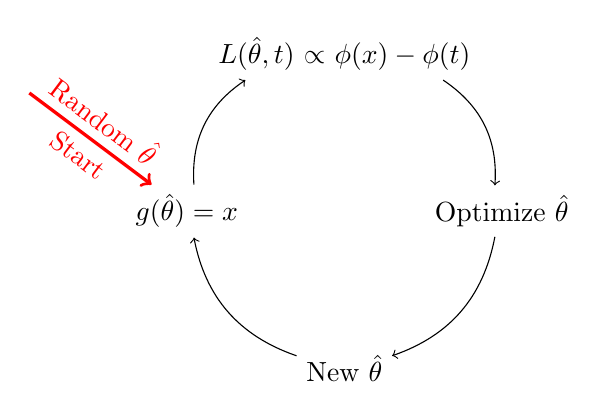
\begin{tikzpicture}[node distance=2cm, auto]

    % Nodes
    \node (start) [text centered] {\( g (\hat{\theta}) = x \)};
    \node (L) [above of=start,right of=start, text centered] {\( L(\hat{\theta},t) {\ \propto \ } \phi(x) - \phi(t) \)};
    \node (optimize) [below of=L,right of=L, text centered] {Optimize $\hat{\theta}$};
    \node (new_theta) [below of=optimize,right of = start, text centered] {New \( \hat{\theta} \)};

    % Highlight and arrow for the start node
    \draw[->, very thick, red] (start) ++(-2,1.5) -- (start)
        node[midway, below, align=center, sloped, color=red] {Start}
        node[midway, above, align=center, sloped, color=red] {Random $\hat{\theta}$};
        
    % Arrows with multi-line labels
    \draw[->, bend left] (start) to node[midway, right, align=center] {} (L);
    \draw[->, bend left] (L) to node[midway, right, align=center] {} (optimize);
    \draw[->, bend left] (optimize) to node[midway, below, align=center] {} (new_theta);
    \draw[->, bend left] (new_theta) to node[midway, left, align=center] {} (start);

\end{tikzpicture}
    % \caption{ Iterative approach to sound design. Synthesizer $g$ with arbitrary initialized parameters $\hat{\theta}$, creates sound $x$. The target sound $t$ is used as the goal. Parameters $\hat{\theta}$ are adjusted to minimize error (or loss) $L(\hat{\theta},t)$, where $L$ is proportional to the difference between the representations of $x$ and $t$. $\phi$ is the audio feature extractor, or representation function.}
    \caption{ Iterative approach to sound design.}
    \label{fig:sound_design_loop_iterative}
\end{figure}

In the upcoming ``Past Works'' section, we will discuss the evolution of prior sound-matching research, with \textit{differentiable iterative sound-matching} being the latest extension of the field.


\begin{table*}[t]
\centering
\caption{Summary of select works in sound-matching. Gen. refers to whether the generations are done in 1-shot (generally, output by a neural network) or a search is conducted with the goal of iteratively getting closer to the target sound.}
\setlength{\tabcolsep}{3pt} % Reduce horizontal spacing
\renewcommand{\arraystretch}{1.05} % Reduce vertical spacing
\scriptsize % Reduce font size
\resizebox{\textwidth}{!}{
\begin{tabular}{|>{\raggedright\arraybackslash}m{2cm}|>{\raggedright\arraybackslash}m{2cm}|>{\raggedright\arraybackslash}m{2cm}|>{\raggedright\arraybackslash}m{2cm}|>{\raggedright\arraybackslash}m{1.2cm}|>{\raggedright\arraybackslash}m{1.2cm}|>{\raggedright\arraybackslash}m{1cm}|>{\raggedright\arraybackslash}m{1cm}|}
\hline
\textbf{Work} & \textbf{Synthesis} & \textbf{Loss} & \textbf{Heuristics} & \textbf{Goal} & \textbf{Domain} & \textbf{Year} & \textbf{Gen. } \\
\hline
Horner \textit{\textit{et al.}}~\cite{horner1993machine} & Non-diff FM & STFT (McAulay-Quatieri) & Direct & Replicate & In & 1991 & Iter \\
\hline
Mitchel \textit{\textit{et al.}}~\cite{mitchell2007evolutionary} & Non-diff FM & Spectral Relative & Evolutionary & Replicate & In (Contrived) & 2007 & Iter \\
\hline
Yee-King \textit{\textit{et al.}}~\cite{yee2018automatic} & Non-diff VST & P-Loss (for Supervised), Spectral (MFCC) & Supervised \& Evolutionary & Replicate & In & 2018 & Both \\
\hline
Esling \textit{\textit{et al.}}~\cite{esling2019flow} & Non-diff VST & Spec MSS/SC P-loss & Supervised \& Modeling & Replicate & In* \& Out & 2019 & 1-shot \\
\hline
Shier \textit{\textit{et al.}}~\cite{shier2020spiegelib} & Custom, non-diff & FFT \& Spectral & Supervised \& Direct & Replicate & In & 2020 & Both \\
\hline
Salimi \textit{\textit{et al.}}~\cite{salimi2020make} & Non-diff & STFT and Envelope & Supervised & Imitate & Out & 2020 & 1-shot \\
\hline
Masuda \textit{\textit{et al.}}~\cite{masuda2021soundmatch} & DDSP & P-Loss initially, fine-tune with Spec. & Supervised & Both & In \& Out & 2021 & 1-shot \\
\hline
Han \textit{\textit{et al.}}~\cite{han2023perceptual} & NN-encoder $\rightarrow$ physical model & PNP (approx. of STFT) & Supervised & Replicate & In & 2023 & 1-shot \\
\hline
Vahidi \textit{\textit{et al.}}~\cite{vahidi2023mesostructures} & Differentiable FM & JTFS/MSS & Direct (grad desc.) & Replicate & In & 2023 & Iter \\
\hline
Uzrad \textit{\textit{et al.}}~\cite{uzrad2024diffmoog} & DDSP chains & Synth. Chain and P-loss & Supervised & Replicate & In \& Out & 2024 & 1-shot \\
\hline
\end{tabular}
}

\label{tab:summary}
\end{table*}

\section{Past Works}
\label{sec:related_works}
Table~\ref{tab:summary} contains an overview of relevant literature, covering important works in sound-matching. Earlier works in this domain focused on FM synthesis and genetic algorithms (or direct optimization methods)\cite{justice1979analytic,horner1993machine,mitchell2007evolutionary}. Along with the exponential increase in computation power, later works utilized a wider range of approaches to parameter search, estimation, and audio synthesis; particularly with supervised learning and neural networks (\gls{NN})~\cite{yee2018automatic,engel2020ddsp,esling2019flow}. 

\subsection{Earlier Works}
FM synthesizers are simple to implement, yet very expressive~\cite{chowning1973synthesis}. Perhaps the earliest foundational work in sound-matching is the analytical approach by Justice~\cite{justice1979analytic} toward the decomposition and recreation of sounds with FM synthesis using one carrier, one modulator, and the corresponding envelopes:
\[ f(t) = I_c(t) \cos(\omega_c t + I_m(t) \cos(\omega_m t))
\]
Where $f(t)$ is the output signal, $I_c(t)$ is the carrier amplitude, $\omega_c$ is the carrier frequency, and $I_m(t)$ and $\omega_m$ are the envelope and frequency for the modulator~\cite{justice1979analytic}.  

 The sound-matching works that followed used other heuristics for finding the synthesizer parameters, yet the simple FM synthesizer structure remained unchanged. Horner \textit{et al.}~\cite{horner1993machine} used GAs for re-synthesis of sounds with an FM synthesizer using one modulator and one carrier oscillator, and the McAulay-Quatieri method~\cite{mcaulay1986speech} for measuring loss. 
 
 % MQ calculates the STFT and marks the start and end of \textit{trends} in a sound with the assumption that the harmonic content belongs to trends that have a beginning and an end. 

Introduction of more complex models of synthesis such as wavetables~\cite{horner2003auto} and physical modeling~\cite{riionheimo2003parameter} rendered interesting results, but led to further questions about the nature and goals of sound-matching. Mitchell and Creasy noted the difficulty in distinguishing between ``inefficiency of the optimization engine'' and ``synthesizer limitations'' as the cause of failure or success in sound-matching~\cite{mitchell2007evolutionary}. They offered a \textit{contrived methodology} for finding the best evolutionary method for sound-matching using their FM synthesizer. The methodology postulates that the best search heuristic for in-domain search (where an exact target exists, and a wide range of targets can be produced by sampling from different points in the parameter space) would also be the best-performing heuristic for out-of-domain search on a dataset of muted trumpet tones~\cite{opolko1989mcgill}; however, testing was not extensive and yielded some contradictory results. As they noted, modifications to the synthesizer, loss function, and sound domain would lead to a problem with an entirely new search space~\cite{mitchell2007evolutionary}. 

% Testing sound-matching experiments can be difficult, in part due to the large number of parametric components and navigation of complex non-linear systems. The issue with finding the best approaches to sound-matching is exacerbated when slight changes to the pipeline render previous results moot. Perhaps due to these reasons, the contrived methodology was not extensively tested by Mitchell and Creasy, who only provided a single experiment where the best evolutionary strategy found by in-domain search would also perform well in out-of-domain synthesis.
\subsection{Introduction of Deep-Learning}
Recent years have seen more works in sound-matching using machine learning techniques. In 2018, Yee-King \textit{et al.} rendered 60,000 audio-parameter pairs from the \textit{Dexed} \gls{VST} synthesizer~\footnote{https://asb2m10.github.io/dexed/}, and showed that NNs trained on this dataset can outperform GA and hill-climber (\gls{HC})~\cite{hoffmann2000heuristic} methods in rendering speed, with slight improvements in MFCC error (used as an objective performance test). The speed improvement appears trivial, considering the iterative nature of GAs when compared to offline training of supervised models. For GAs and HC optimizer, MFCCs were used as a measure of performance as well as a loss function. For training the networks, P-loss was used, since differentiable MFCCs were not possible in their pipeline. Importantly, informal hearing tests revealed that the performance of even the best NN model was unsatisfactory, possibly due to the complex nature of the synthesizer, which features 155 parameters.


% Programming synthesizers and querying sounds by imitating human vocals has also been a subject of interest~\cite{Cartwright2014SynthAssistQA,siamesevocalimitation2018}. For example, Cartwright and Pardo created a framework for searching pre-made patches for a synthesizer to best imitate vocals using audio features such as pitch, spectral centroid, and loudness~\cite{Cartwright2014SynthAssistQA}. 

Esling \textit{et al.} noted the issue of using P-Loss in sound-matching~\cite{esling2019flow}, considering the non-linear mapping between parameters of a synth and the audio output. In their approach, dubbed as ``flowsynth'', they used a large parameter-to-audio dataset for a commercial \gls{VST} synthesizer. In flowsynth, audio is encoded to an auditory space, using a NN autoencoding approach~\cite{hinton2006reducing}. The encodings in the auditory space can then be converted to the parameter space, but only for that particular synthesizer. Using P-Loss and Spectral Convergence (Frobenius norm of the spectrograms) as metrics, flowsynth outperformed other NN approaches that did not use an auditory to parameter space conversion, but formal hearing tests were not conducted.

Masuda \textit{et al.} also applied supervised learning to synthesizer parameter estimation~\cite{masuda2021soundmatch}. Their work highlights the issue of non-linearity in parameter-to-synthesizer outputs and out-of-domain search. This work uses a differentiable subtractive synthesizer (two oscillators and an LP filter). A NN model was pre-trained using an in-domain dataset of randomly selected parameters and P-Loss. After training, the model was fine-tuned using 20,000 out-of-domain sounds from the NSynth dataset~\cite{engel2017neural} and multi-scale spectrogram loss~\cite{engel2020ddsp}. This approach proved more effective---that is, lower multi-level spectral difference in out-of-domain tests---than baseline models, which were either not exposed to out-of-domain sounds or trained exclusively with P-Loss. Subjective hearing tests were conducted, showing a preference for the fine-tuned model~\cite{masuda2021soundmatch}. Masuda \textit{et al.} later extended this work with semi-supervised learning, highlighting significant gaps in in-domain and out-of-domain performance~\cite{masuda2023improving}.

Rather than focusing on a particular implementation, Shier \textit{et al.} presented Spieglib, a library for implementation of sound-matching pipelines~\cite{shier2020spiegelib}. This library provides different choices for DNNs, GAs, synthesizers, and feature extractors. Shier \textit{et al.} presented an experiment with a similar setup to Yee-King \textit{et al.}~\cite{yee2018automatic}, however, they found a genetic algorithm to be the best performing.

% Rather than focusing on a particular implementation, Shier \textit{et al.} presented Spieglib, a library for implementation of sound-matching pipelines (which Shier \textit{et al.} referred to as ``automatic parameter search'')~\cite{shier2020spiegelib}. This library provides extensible choices of deep-learning estimators with \textit{tensorflow}~\cite{abadi2016tensorflow}, genetic estimators with \textit{DEAP}~\cite{DEAP_JMLR2012}, feature extractors with \textit{librosa}~\cite{mcfee2015librosa}, and different choices for synthesizers, evaluators, dataloaders. Shier \textit{et al.} provide an example experiment using this library. This example has a setup similar to Yee-King \textit{et al.}~\cite{yee2018automatic}, where the \textit{Dexed} VST was used and different genetic and NN estimators were compared by using MFCC difference as the minimization objective. Depending on the NN architecture, MFCC or STFT spectrograms were used as the input. Unlike previous comparisons of NN and genetic algorithms, the best estimator was the multi-objective non-dominated sorting genetic algorithm III (NSGA-III). This algorithm had multiple minimization objectives: 13-band MFCC, STFT, and five spectral features. Shier \textit{et al.} report that all models performed relatively well at imitation of harmonic distributions, but the multi-objective function was the only optimizer which did \textit{not} struggle with matching temporal envelopes of the audio spectrum~\cite{shier2020spiegelib}.


Differentiable loss functions that use spectrogram differences can be computationally expensive. To mitigate this, Han \textit{et al.}~\cite{han2023perceptual} introduced ``perceptual-neural-physical loss'' (PNP). PNP is an approximation of loss functions; specifically, a loss function that uses the L2 norm of the difference between the features of two sounds, or $||\phi(t) - \phi(x)||^2_2$, where $\phi$ could be a spectrogram or JTFS function. PNP loss functions are fast and differentiable, but require training and parameter estimation. A Riemannian metric M needs to be calculated for the minimization of locally linear approximation of the ``true" spectral loss function~\cite{han2023perceptual}. 
\[
\|\phi(t) - \phi(x)\|_2^2 = \langle \tilde{\theta} - \theta | \mathbf{M}(\theta) | \tilde{\theta} - \theta \rangle + O(\|\tilde{\theta} - \theta\|_2^3). \tag{4}
\]

During the training phase, this metric is calculated alongside the neural parameter estimator. After training, PNP can be used as a fast approximation of computationally demanding loss functions such as JTFS~\cite{han2023perceptual,han2024learning}, paired with FM synthesizers and a differentiable physical model of a drum head~\cite{smith2010physical}.

Uzrad \textit{et al.}~\cite{uzrad2024diffmoog} took another unique approach to sound-matching: using a differentiable \textit{synthesis chain} of DSP generators and effects and a loss function that combines P-Loss with a \textit{signal-chain loss}. The synthesizer is a customizable chain of effects, which feed one output as input to the next step of the chain; signal-chain loss compares the parameter and output difference at every output step in the chain~\cite{uzrad2024diffmoog}. Possible chain functionalities are FM/AM, Low-Frequency Oscillators (\gls{LFO}), filters, and envelopes. Like the results shown by Masuda \textit{et al.}~\cite{masuda2021soundmatch}, better out-of-domain results were achieved when pre-trained on in-domain data and fine-tuned using out-of-domain NSynth data~\cite{engel2017neural}. 

% Uzrad \textit{et al.}\cite{uzrad2024diffmoog} used log-spectral distance (LSD) as their loss function, where   
% $\text{LSD} = \| \log(S(t)) - \log(S(x)) \|_F$, S is the mel-spectrogram of the sounds and F is the Frobenius norm~\cite{golub2013matrix}. The Frobenius norm of a matrix $A$ is defined as
% $ \|A\|_F = \sqrt{\sum_{i,j} |a_{ij}|^2}$. Here, $A$ would be the 2D matrix resulting from subtracting two log-spectrograms. Along with other works, \textbf{non-convexity of loss surfaces when applying gradient optimization} is a noted issue~\cite{turian2020sorry,vahidi2023mesostructures,uzrad2024diffmoog}. 

\subsection{What is Lacking In the Field}
\label{sec:lacking}
%   % First, we need to clearly define the characteristics we are looking for with non-generic loss functions, otherwise the chances of finding the sound(s) of interest is slim. Second, we need to move beyond direct replication, and focus on imitating target sounds that are outside the synthesizers capabilities. Third, more complex methods of synthesis need to be explored for iterative sound-matching. Fourth, we need to find optimization methods that can effectively navigate the the sinusoidal nature of loss function landscapes. 

% Based on the literature reviewed, we find several gaps in past research that makes the application of sound-matching for sound-designers difficult. Thus far, replication of in-domain sounds has been the main subject of research. With in-domain replication, we already have the target sound \textit{and} the program that makes it. This simplifies the problem of measuring performance and is the reason why this type of sound-matching research is by far the most common. However, practical application of sound-matching requires answers to much harder problems. Sound-matching would be an interesting creative tool if we could use it to either:
% \begin{enumerate}
%  \item \textbf{Replicate out-of-domain sounds}: this would give us the parameters that could closely approximate a target sound, and we can modify the sound further by modulating the synthesizer. 
% \item \textbf{Imitate in-domain or out-of-domain sounds}: This would allow for applying the characteristics of one sound to another. 
% \end{enumerate}

% We need to be aware of the ``open set recognition'' (\gls{OSR}) problem here \cite{mundt2019open,gers2000learning}. OSR is a well documented issue in DL that manifests when the set or category that the network is supposed to reject or accept cannot be explained via examples. With imitation or replication of out-of-domain sounds, we can expect issues related to OSR to occur, since target and output sounds would be from different domains~\cite{salimi2021percussive}. 

% Perhaps one method of addressing the OSR problem is the use of representations (or feature extraction) methods that reduce sounds to a feature vector in the same domain. For example, a representation that only looks at the envelope of sounds is far less likely to be subject to the OSR problem. \textcolor{highlight}{We highlight the lack of non-generic loss functions as a major weakness in previous works and an interesting area to explore}. 

% Another weakness \textcolor{highlight}{is that the synthesis methods in past works are not representative of the common methods used by sound designers and modern synthesizers}. Simple FM/AM synthesizers have generally been the go-to methods of sound-matching. We believe that general statements regarding the effectiveness of an approach to iterative sound-matching (particularly in regards to a loss function) can only be reasonably made in the context of the subset of the tested methods of synthesis.
% \textcolor{highlight}{The simplicity of parameter optimization approaches} is another area of weakness in past works. Classic genetic algorithms update the parameters randomly, while in recent differentiable settings, simple gradient descent methods are used. Past works have provided issues which arise in differentiable parameter estimation due to periodic loss functions. Perhaps the use of reinforcement learning (\gls{RL}), or other algorithms that continually learn from their environment, could help with this problem.

% \subsection{Defining The Major Issues}
% \label{sec:addressing_problems}

Having looked at the current available literature, we note four major areas of weakness in sound-matching. We target the first two issues in this work, while the latter two issues are left for future work. 
\begin{enumerate}
    \item \LossSelect: Is there a \textit{best performing} loss function, or is the selection of the loss function dependent on factors such as the sound domain, synthesizer capability and the desired characteristics of the output? 
    \item \SynthSelect: There is a lack of diversity in the synthesis methods used in sound-matching. The use of different DSP functions for iterative sound-matching and their effects on the outcome or the interactions with the loss function have not been tested.
    \item \PeriodicLoss: The sinusoidal nature of loss function landscapes is a problem that appears frequently. In differentiable settings, this problem causes gradient descent updates to local minima. 
    \item \OutDomain: Sound-matching with out-of-domain sounds is an unexplored area, yet a necessary one for practical applications for sound designers.
\end{enumerate}

\section{Programs, Methodology, and Results}
\label{sec:progs_methodology_results}
Towards addressing the problems of \LossSelect{} and \SynthSelect{}, we compare the performance of iterative sound-matching experiments, where four differentiable loss functions are applied to four differentiable synthesizers. What we mean by ``performance'' is the similarity of the final output to the target, as measured by P-Loss, MSS, and---most importantly---manual listening tests.

\textbf{We hypothesize that the relative performance of loss functions for sound-matching is influenced by the method of synthesis}. If true, this would strengthen the idea that the selection of the loss function and synthesis method is not an optimization problem, but a subjective choice depending on the needs of the sound designer. 

% In Section~\ref{sec:methodology} we lay out the experiment methodology. Section~\ref{sec:loss_implementation} discusses the details of implementation for the loss functions. Section~\ref{sec:programs} covers the characteristics of the programs, and finally Section~\ref{sec:results_posthoc} shows that the effect of loss function choice on the success of iterative sound-matching is dependent on the signal process chain of interest. 

\subsection{Experiment Methodology}
\label{sec:methodology}
% We have highlighted the lack of attention given to the selection of loss functions in sound-matching, and noted that the few existing works addressing this issue evaluate their proposed losses using only simplistic sound synthesis methods. \textcolor{highlight}{We hypothesize that the best performing loss function is influenced by the synthesis techniques utilized in the synthesizer}. This hypothesis targets the issues of \LossSelect~and \SynthSelect. 

We test four different loss functions and compare their success in sound-matching using four different synthesizers. We verify the success of the sound-matching process using two automatic measures of sound similarity (MSS and P-Loss) and a manual blinded hearing test conducted by two of the authors where Likert scores~\cite{jebb2021review} of 1-5 are assigned to a subset of final outputs and the corresponding targets.

An \textit{experiment} is one iteration of sound-matching given a loss function, target sound,
and synthesizer program. When the final iteration is complete, a score is given (automatically with an algorithm or with manual listening) to an experiment that measures its success in replicating the target sound. Consider the following simplified scenario: we have two loss functions, $L_1$ and $L_2$, and a single synthesizer program $P$ with a target parameter set $\theta^*$ where the target sound is $t$, or $P(\theta^*) = t$. We run a large number (in this case, 300 for each loss function) of experiments where we randomly set the initial ($\theta_0$) and target parameters ($\theta^*$) of $P$ and run an iterative sound-matching loop for each loss function, with maximum number of iterations set to 200. When the loop is terminated, we measure the similarity of the final output sound $x$ (where $P(\theta_{199}) = x$) to $t$, or if using P-Loss we compare $\theta_{199}$ to $\theta^*$. Having 300 experiments gives us a distribution of losses to determine whether $L_1$ or $L_2$ led to better performance. This simplified example leads us to our methodology which has four loss functions, four synthesizer programs, and three different evaluation methods of scoring sound similarity.

\subsubsection{Automatic and Manual Evaluation}
\label{sec:evaluation_manual_auto}
The two automatic evaluation methods used here are P-Loss and MSS, as described in Section~\ref{sec:loss_funcs}. For P-Loss, the parameters are normalized between 0-1 based on the valid ranges defined in the Faust program, and the L1 distance between the normalized parameters is calculated. MSS is computed using a hop size of $100$ samples, and FFT window lengths of $(512, 1024, 2048, 4096)$. 

Automatic sound evaluation methods are often unreliable, as their alignment with the subjective judgments of human listeners is uncertain. Therefore, listening tests are conducted by randomly sampling 40 experiment results for each program and loss function pair. Two of the authors then assign blinded similarity scores to the outputs and targets using a 5-point Likert scale (1 = no similarity, 5 = near identical)~\cite{jebb2021review}. Using Spearman's rank correlation~\cite{spearman1987proof,rebekic2015pearson}, we found a very strong rate of agreement between the human listeners (see Section~\ref{sec:consistency_in_rankings}), a good indicator that the scores assigned by manual listeners can be treated as the ground truth. We then combine the ranks assigned by both authors, giving us 80 ranks per program and loss function pair. 


% Agreement between the assigned scores is measured using Spearman’s rank correlation, which provides both a correlation coefficient ($\rho$) ranging from –1 (perfect negative correlation) to 1 (perfect positive correlation), and a p-value testing the null hypothesis of no correlation~\cite{spearman1987proof,rebekic2015pearson}. Across all programs, the correlation was very strong ($\rho = 0.86$, $p < 10^{-180}$). Per-program correlations were also very strong: $\rho = 0.71$ for \BPNoise{} ($p < 10^{-25}$), $\rho = 0.64$ for \AddSineSaw{} ($p < 10^{-19}$), $\rho = 0.84$ for \AmpMod{} ($p < 10^{-43}$), and $\rho = 0.85$ for \FMMod{} ($p < 10^{-44}$). This high rate of agreement is a good indicator that the scores assigned by manual listeners can be treated as the ground truth. 

% For each program and loss function, the blind manual hearing test gives us 80 ranks, which are given by two of the authors to a set of 40 randomly selected experiment results. This gives 160 pairs of ranks per program, and 640 for all programs. We computed Spearman correlations between the two reviewers.

\subsubsection{Determining Best Performers}
 Figure~\ref{fig:posthoc_evaluation} is a visualized summary of how the loss functions are ranked. We have four loss functions and four synthesizer programs. The maximum number of iterations set to 200, and 300 experiments for each loss/synthesizer combination. Each synthesizer program is paired with four loss functions and 300 experiments are conducted and evaluated automatically with P-Loss and MSS. Two of the authors assigned blinded Likert scores to 40 randomly selected sounds, where integers from 1 to 5 are assigned, with 1 meaning no similarity and 5 for near identical. 

For each program and loss function pair, we have three distributions that can be used to rank the loss functions. Two with 300 automatically assigned similarities (P-Loss and MSS) and one with 80 Likert scores (combining the 40 ranks assigned by each author). For consistency and statistical robustness, the distributions are upsampled to 1000 values using bootstrapping~\cite{tibshirani1993introduction}. Bootstrapping gives an estimation of the distribution for the mean performance of each experiment. $k$ (set to 1000) samples of $n$ values (set to 100\% of the values) are taken with replacement from the empirical distribution (list of 300 performance values for MSS and P-Loss or 80 for manual rankings). The mean performance is calculated for each of the $k$ samples. The $k$ estimates of the mean performance give us a bootstrapped distribution for each loss function. 

For each program, the loss functions are ranked using the non-parametric Scott-Knott (\gls{NPSK}) test~\cite{tantithamthavorn2017mvt,tantithamthavorn2018optimization}, which ranks the loss functions from rank 1 (best, or highest distribution values) to maximum rank of 4 (worst, with lowest distribution values). NPSK may determine that multiple functions belong to the same rank, in which case the maximum rank would be less than 4. As mentioned before, lower P-Loss and MSS values indicate higher similarity, therefore (for consistency with manually assigned ranks) the reciprocal of their output is used ($x^{-1}$, if $x$ is the P-Loss or MSS value), where higher values indicate greater similarity. 


\begin{figure*}
\resizebox{\linewidth}{!}{ % Automatically scales diagram to fit page width
\begin{tikzpicture}[
    function/.style={rectangle, draw, rounded corners, minimum width=2cm, minimum height=1cm, text centered, node distance=1.5cm},
    distribution/.style={ellipse, draw, minimum width=2cm, minimum height=1cm, text centered, node distance=1.2cm},
    gaussian/.style={draw, smooth, samples=100, domain=-2.5:2.5},
    snpk/.style={rectangle, draw, rounded corners, minimum width=2.5cm, minimum height=1cm, text centered, node distance=1.5cm, fill=blue!20},
    level 1/.style={sibling distance=6cm, level distance=2cm},
    level 2/.style={sibling distance=2cm, level distance=3cm},
    mss/.style={fill=red!50, draw=black},
    ploss/.style={fill=blue!50, draw=black},
    likert/.style={fill=green!40, draw=black}
]

% Existing functions and distributions diagram
\node[function] {Synthesizer Program}
    child { node[function] {DTW\_Onset}
        child { node[distribution, mss] {MSS}
            child[grow=down, level distance=1.5cm] {
                node[draw=none] {
                    \begin{tikzpicture}[scale=0.7]
                        \draw[red] plot (\x/3, {exp(-\x*\x)});  % Red Gaussian
                    \end{tikzpicture}
                }
            }
        }
        child { node[distribution, ploss] {P-Loss}
            child[grow=down, level distance=1.5cm] {
                node[draw=none] {
                    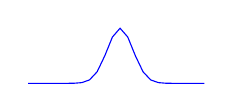
\begin{tikzpicture}[scale=0.7]
                        \draw[blue] plot (\x/3, {exp(-\x*\x)});  % Blue Gaussian
                    \end{tikzpicture}
                }
            }
        }
        child { node[distribution, likert] {Likert}
            child[grow=down, level distance=1.5cm] {
                node[draw=none] {
                    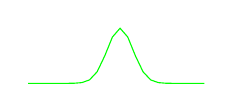
\begin{tikzpicture}[scale=0.7]
                        \draw[green] plot (\x/3, {exp(-\x*\x)});  % Green Gaussian
                    \end{tikzpicture}
                }
            }
        }
    }
    child { node[function] {L1\_Spec}
        child { node[distribution, mss] {MSS} }
        child { node[distribution, ploss] {P-Loss} }
        child { node[distribution, likert] {Likert} }
    }
    child { node[function] {SIMSE\_Spec}
        child { node[distribution, mss] {MSS} }
        child { node[distribution, ploss] {P-Loss} }
        child { node[distribution, likert] {Likert} }
    }
    child { node[function] {JTFS}
        child { node[distribution, mss] {MSS}
            child[grow=down, level distance=1.5cm] {
                node[draw=none] {
                    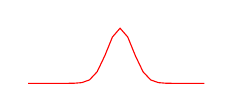
\begin{tikzpicture}[scale=0.7]
                        \draw[red] plot (\x/3, {exp(-\x*\x)});  % Red Gaussian
                    \end{tikzpicture}
                }
            }
        }
        child { node[distribution, ploss] {P-Loss}
            child[grow=down, level distance=1.5cm] {
                node[draw=none] {
                    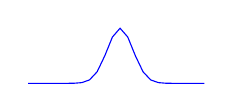
\begin{tikzpicture}[scale=0.7]
                        \draw[blue] plot (\x/3, {exp(-\x*\x)});  % Blue Gaussian
                    \end{tikzpicture}
                }
            }
        }
        child { node[distribution, likert] {Likert}
            child[grow=down, level distance=1.5cm] {
                node[draw=none] {
                    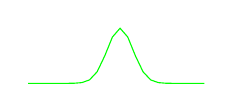
\begin{tikzpicture}[scale=0.7]
                        \draw[green] plot (\x/3, {exp(-\x*\x)});  % Green Gaussian
                    \end{tikzpicture}
                }
            }
        }
    };

% Label for the second row (Distributions)
\node at (0,-6.5) {\textbf{$\longleftarrow$\ \ \large Bootstrapped Distributions\ \ $\longrightarrow$}};

% Left side: SNPK with MSS
\node[snpk, text height=5ex, align=center, fill=red!30, draw=black] at (-6,-9) {SNPK with 4 \\ MSS distributions};
\draw[->] (-6,-9.5) -- (-6,-10.5) node[below, below] {\textbf{Ranks 1-4}};
\draw[red!40, thick] (-4.5, -8.4) -- (-2.75, -7.75);  % Line 1
\draw[red!40, thick] (-5.25, -8.4) -- (-3.5, -7.75);  % Line 2
\draw[red!40, thick] (-5.75, -8.4) -- (-5.5, -7.75);  % Line 3
\draw[red!40, thick] (-6.25, -8.4) -- (-9, -7.75);  % Line 4

% Middle: SNPK with P-Loss
\node[snpk, text height=5ex, align=center, fill=blue!40, draw=black] at (0,-9) {SNPK with 4 \\ P-Loss distributions};
\draw[->] (0,-9.5) -- (0,-10.5) node[below, below] {\textbf{Ranks 1-4}};
\draw[blue!40, thick] (1.5, -8.4) -- (3.25, -7.75);  % Line 1
\draw[blue!40, thick] (0.75, -8.4) -- (1.5, -7.75);  % Line 2
\draw[blue!40, thick] (-0.25, -8.4) -- (-1, -7.75);  % Line 3
\draw[blue!40, thick] (-0.75, -8.4) -- (-3, -7.75);  % Line 4

% Right side: SNPK with Likert
\node[snpk, text height=5ex, align=center, fill=green!30, draw=black] at (6,-9) {SNPK with 4 \\ Likert distributions};
\draw[->] (6,-9.5) -- (6,-10.5) node[below, below] {\textbf{Ranks 1-4}};
\draw[green!50, thick] (7.5, -8.4) -- (8.75, -7.75);  % Line 1
\draw[green!50, thick] (6.75, -8.4) -- (6, -7.75);    % Line 2
\draw[green!50, thick] (6.25, -8.4) -- (4, -7.75);   % Line 3
\draw[green!50, thick] (5.75, -8.4) -- (3, -7.75);     % Line 4

\end{tikzpicture}
}
\caption{For each synthesizer program, we assign ranks to the four loss functions  (\DTWEnv, \LoneSpec, \SIMSESpec, \JTFS) in three different ways, using MSS, P-Loss, or manually assigned Likert scores.}
\label{fig:posthoc_evaluation}
\end{figure*}

\subsubsection{Training Parameters and Gradient Calculations}
 % Previous work utilized gradient fields for analysis of the algorithm performance~\cite{vahidi2023mesostructures}. Gradient fields are not the center of our analysis, but we include them in Appendix~\ref{appendix:gradient_fields}.
 For updating the synthesizer parameters (or weights), we use RMSProp, which operates similar to stochastic gradient descent (SGD)~\cite{goodfellow2016deep}, with the caveat that the gradients of each weight are scaled by the root-mean-square of past gradients of that weight. Based on some initial test runs, we used an arbitrary fixed learning rate of 0.045 for all experiments (learning rates used in Vahidi \textit{et al.}~\cite{vahidi2023mesostructures} is unknown). The maximum number of iterations is set to 200, where, based on our observations, the parameters have either irrecoverably diverged outside the acceptable ranges, or are stuck at a local minimum. Additionally, the gradients are large, and calculated backwards sequentially through the signal processing chain. This backward calculation resembles the \textit{exploding gradients} problem in recurrent neural networks~\cite{gers2000learning}. Gradient clipping~\cite{goodfellow2016deep} is preemptively used to ensure that the  $\ell_2$ norm of all gradients does not exceed the threshold of 1. 
% \mathbf{\gamma}_i^{\text{clipped}} = \mathbf{\gamma}_i \cdot \mathcal{S}
% \]
% Where $\mathcal{S}$ is a value less than or equal to 1, depending on whether the norm of the gradients exceeds the threshold $c$.  
% \[
% \mathcal{S} = \frac{c}{\max(\|\mathbf{\gamma}\|_2, c)}
% \]


\subsection{Loss Function Implementation Details}
\label{sec:loss_implementation}
\subsubsection{STFT Losses}
Due to their ubiquity and lower cost of gradient calculation, we use STFT as the basis of two of the loss functions. As discussed in Section~\ref{sec:matching_types}, the L1 or L2 distances are the most common methods of comparing different spectrograms, however, there are situations where this might lead to shortcomings. An example given by Vahidi \textit{et al.}~\cite{vahidi2023mesostructures} is two chirplets (tones that increase in pitch) starting and ending at the same frequencies. If one of these tones is slightly shifted in time, then the spectrograms will no longer overlap at any point, despite their sonic similarity. In this example, we do not know if this is an issue of the spectrograms, or the L1 measure used for their comparison. In the computer vision field, Structural Similarity Index (SSIM)~\cite{wang2004imagesssim,wang2009mean} and Scale-Invariant Mean Squared Error (SIMSE)~\cite{barron2014shapessimse} have been used as alternatives that improved performance in various tasks relative to L1.

We define the \LoneSpec~and \SIMSESpec~functions as the application of L1 and SIMSE to the STFT spectrograms. The STFT spectrogram function uses 512 FFT bins, window size of 600 samples, and hop length (how many samples the window shifts) of 100 samples. The L1 and SIMSE implementations are differentiable. 

\subsubsection{JTFS Loss}
The \JTFS~loss function is the application of L1 difference to the JTFS representations of two sounds~\cite{vahidi2023mesostructures}. The code used for the JTFS transformation is the differentiable implementation of a 1-dimensional JTFS function provided by Andreux \textit{et al.}~\cite{kymatio}.

\subsubsection{Soft-DTW Loss}
We use the soft-DTW function, which is differentiable and --- depending on its parameters --- not shift-invariant~\cite{cuturi2017soft,janati2020spatio,tavenard.blog.softdtw}. The loss function \DTWEnv~is the application of the soft-DTW function to the envelope of the two sounds being compared~\cite{lyons1997understanding}. The envelope is calculated by creating the STFT spectrogram of a sound (the same process used in Section~\ref{sec:fourier_specs}) and summing the values at each timestep. 

\subsection{The Synthesizers}
\label{sec:programs}
The synthesizer programs are meant to be simple examples that test the building blocks of digital sound synthesis. Subtractive, additive, and FM/AM synthesis are three of the most common techniques in sound design~\cite{smith1991viewpoints}. In subtractive synthesis, frequencies are removed from a sound via digital filters. In additive synthesis, complex sounds are created via the linear combination of simpler sounds~\cite{lyons1997understanding,smith2007introduction}. As discussed previously, FM/AM synthesis refers to the general technique of modulating the frequency or amplitude of a waveform (the carrier) by another waveform (the modulator).

For each program, we provide the Faust code~\cite{orlarey2009faust}, which can be run in the online IDE~\footnote{\url{https://faustide.grame.fr/}}. Faust is a functional language for audio synthesis that can succinctly define signal processing chains. Following Braun's methodology~\cite{braun2024dac}, programs are first defined in Faust, then converted (or \textit{transpiled}) to differentiable Jax functions using the DawDreamer library\footnote{\url{https://github.com/DBraun/DawDreamer}}. 

 Once the programs are transpiled to differentiable synthesizers, the iterative sound-matching procedure is:
 \begin{enumerate}
    \item Initialize $\theta^*$ and $\hat{\theta}$, i.e., random generation of target and initial parameters uniformly over a predefined range
    \item Generating the output of the synthesizer with $\hat{\theta}$ (the length of the output is set to 1 second with sample-rate of 44100 Hz) 
    \item Calculating the loss between the target and output
    \item Applying gradient updates to the synthesizer parameters
    \item Repeating the second step with the updated parameters $\hat{\theta}$, until maximum number of iterations has been reached
 \end{enumerate}

% A general overview of the programs and the predefined parameter ranges is given in Table~\ref{tab:programs}.

In the following subsections, we describe the programs and their parameters in more detail, followed by the methodology in Section~\ref{sec:methodology} and results in Section~\ref{sec:results_posthoc}.

% \begin{table*}[htbp]
% \centering
% \begin{adjustbox}{max width=\textwidth}
% \begin{tabular}{|c|c|c|c|l|}
% \hline
% \textbf{ID} & \textbf{Parameters} & \makecell{\textbf{Param. 1}\\\textbf{Range}} & \makecell{\textbf{Param. 2}\\\textbf{Range}} & \textbf{Description} \\
% \hline
% \BPNoise & hp\_cut, lp\_cut & 50-1000 & 1-120 & Band-pass of Noise signal \\
% \hline
% \AddSineSaw & saw\_freq, sine\_freq & 20-1000 & 20-1000 & Addition of sine and saw waves \\
% \hline
% \AmpMod & amp, carrier & 1-20 & 20-1000 & LFO on amplitude of noise osc \\
% \hline
% \FMMod & amp, carrier & 0-5 & 0-4 & LFO on amplitude of saw osc \\
% \hline
% \end{tabular}
% \end{adjustbox}
% \caption{Overview of Program Parameters and the range of values each parameter can take.}
% \label{tab:programs}
% \end{table*}



\begin{lstlisting}[caption={\BPNoise}, label={lst:program0}, language=Faust,
                  float, floatplacement=!H, xleftmargin=1em, xrightmargin=0.5em, firstnumber=0, aboveskip=0em, belowskip=-1em]
import("stdfaust.lib");
lp_cut = hslider("lp_cut",900,50,1000,1);
hp_cut = hslider("hp_cut",100,1,120,1);
process = no.noise:fi.lowpass(3,lp_cut):fi.highpass(10,hp_cut);
\end{lstlisting}

\begin{lstlisting}[caption={\AddSineSaw}, label={lst:program1},language=Faust,float,floatplacement=!H,xleftmargin=1em,xrightmargin=0.5em,firstnumber=0,aboveskip=0em, belowskip=-1em]
import("stdfaust.lib");
saw_freq = hslider("saw_freq",800,20,1000,1);
sine_freq = hslider("sine_freq",300,20,1000,1);
sineOsc(f) = +(f/ma.SR) ~ ma.frac:*(2*ma.PI) : sin;
sawOsc(f) = +(f/ma.SR) ~ ma.frac;
process = sineOsc(sine_freq)+sawOsc(saw_freq);
\end{lstlisting}

\begin{lstlisting}[caption={\AmpMod}, label={lst:program2},language=Faust,float,floatplacement=!H,xleftmargin=1em,xrightmargin=0.5em,firstnumber=0,aboveskip=0em, belowskip=-1em]
import("stdfaust.lib");
amp = hslider("amp",0.5,0,5,0.01);
modulator = hslider("modulator",0.5,0,4,0.01);
sineOsc(f) = +(f/ma.SR) ~ ma.frac:*(2*ma.PI) : sin;
process = no.noise*sineOsc(modulator)*amp;
\end{lstlisting}

\begin{lstlisting}[caption={\FMMod}, label={lst:program3},language=Faust,float,floatplacement=!H,xleftmargin=1em,xrightmargin=0.5em,firstnumber=0,aboveskip=0em, belowskip=-1em]
import("stdfaust.lib");
carrier = hslider("carrier",100,20,1000,1);
amp = hslider("amp",6,1,20,1);
sineOsc(f) = +(f/ma.SR) ~ ma.frac:*(2*ma.PI) : sin;
sawOsc(f) = +(f/ma.SR) ~ ma.frac;
process = sineOsc(amp)*sawOsc(carrier);
\end{lstlisting}

\subsubsection{\BPNoise}
\label{sec:program0}
\BPNoise{} is a bare bones example of subtractive synthesis using digital filters~\cite{smith2007introduction}. Despite the ubiquity of subtractive synthesis in practical sound design, it has rarely been tested in differentiable sound-matching. In this program, a noise signal is fed through a band-pass (BP) filter. This removes the frequencies outside the low-pass (LP) and high-pass (HP) cutoffs. The noise generator produces all frequencies with random variation over time. The LP filter removes frequencies over its threshold frequency, and the HP removes frequencies lower than its threshold~\cite{smith2007introduction}. The search parameters are the cutoff thresholds for the LP and HP filters. Listing~\ref{lst:program0} shows the Faust code for \BPNoise.

\subsubsection{\AddSineSaw}
\label{sec:program1}
\AddSineSaw{} is an additive program that combines a saw and a sine wave function. Like subtractive synthesis, additive synthesis is a common approach to sound design that has not been extensively tested as a benchmark in sound-matching. The search parameters here are the frequency of the sine and saw oscillators. Listing~\ref{lst:program1} is the Faust code for \AddSineSaw.

\subsubsection{\AmpMod}
\label{sec:program2}
\AmpMod{} involves amplitude modulation of a noise generator by an LFO with \textit{modulator} as its frequency and a global \textit{amp} value that does not change over time and applies to the entire signal. The search parameters for this program are the LFO frequency and the amp value. The amp value acts as a global volume control, and since the sounds are normalized before analysis, it is likely inconsequential to the performance. This program is meant to be a stepping stone to \FMMod, which utilizes proper AM synthesis. Listing~\ref{lst:program2} is the Faust code for \AmpMod. 

\subsubsection{\FMMod}
\label{sec:program3}
Relative to additive and subtractive synthesis, AM/FM synthesis are less common methods of sound design. Due to their frequent use in previous works, we also tested an AM synthesizer. The synthesizer program is the multiplication of a low frequency sine oscillator with frequency parameter \textit{amp}, and a saw oscillator with frequency parameter \textit{carrier}. Listing~\ref{lst:program3} is the Faust code for \FMMod. 

\subsection{Post hoc Analysis of Loss Performance}
\label{sec:results_posthoc}
As summarized in Figure~\ref{fig:posthoc_evaluation}, for each program and evaluation (or scoring) method, there are four sets 1000 bootstrapped values, corresponding to the four loss functions. A post-hoc test is conducted in two stages in order to determine whether there is a difference in performance between loss functions for each program, and if so, which are the best performers. The first stage determines whether there is a difference in group means, with the null hypothesis being that all groups have similar mean ranks. The second stage ranks the loss functions from best to worst using the non-parametric Scott-Knott test (\gls{NPSK})~\cite{tantithamthavorn2017mvt,tantithamthavorn2018optimization}.
The Kruskal-Wallis test is used for the first stage~\cite{kruskal1952use}; this test pools and ranks all evaluation measures for a program, then tests whether the differences in mean rank for all loss function groups is zero. The Kruskal-Wallis test calculates an H statistic that is compared to a chi-square distribution with k-1 degrees of freedom (k is the number of groups, or 4, and degrees of freedom is 3). Using the significance level of 0.05, if the H statistic is greater than the critical value of the chi-square distribution then the null hypothesis is rejected, meaning that at least one group has a mean rank significantly above others~\cite{kruskal1952use}. Table~\ref{tab:kruskal_auto} shows the Kruskal-Wallis results for every program and evaluation method, and shows that significant differences between loss function performance measures (i.e., the bootstrapped distributions of the evaluation for each loss function) exist in all cases except MSS for the \AmpMod{} program. 

\begin{table}[ht]
\centering
\caption{Do loss functions have different median performance? Kruskal-Wallis results by program and bootstrapped evaluation results.}
\begin{tabular}{|c|c|c|c|c|}
\hline
\textbf{Program} & \textbf{Eval. Method} & \textbf{H-Stat.} & \textbf{P-value} & \textbf{Reject} \\
\hline
\BPNoise & MSS      & 81.19  & $1.70 \times 10^{-17}$ & Yes \\
\BPNoise & P-Loss  & 163.60 & $3.07 \times 10^{-35}$ & Yes \\
\BPNoise & Manual & 9.45  & $2.39 \times 10^{-2}$ & Yes \\
\AddSineSaw & MSS      & 308.97 & $1.14 \times 10^{-66}$ & Yes \\
\AddSineSaw & P-Loss  & 348.42 & $3.28 \times 10^{-75}$ & Yes \\
\AddSineSaw & Manual & 9.45  & $2.39 \times 10^{-2}$ & Yes \\
\AmpMod & MSS      & 1.35   & $0.7171$               & No \\
\AmpMod & P-Loss  & 366.76 & $3.50 \times 10^{-79}$ & Yes \\
\AmpMod & Manual & 32.71 & $3.70 \times 10^{-7}$ & Yes \\
\FMMod & MSS      & 564.65 & $4.65 \times 10^{-122}$ & Yes \\
\FMMod & P-Loss  & 229.19 & $2.07 \times 10^{-49}$ & Yes \\
\FMMod & Manual &  207.58 & $9.69 \times 10^{-45}$ & Yes \\
\hline
\end{tabular}
\label{tab:kruskal_auto}
\end{table}

% \begin{table}[ht]
% \centering
% \begin{tabular}{|c|c|c|c|}
% \hline
% \textbf{Program} & \textbf{H-Stat.} & \textbf{P-value} & \textbf{Reject} \\
% \hline
% \BPNoise & 9.45  & $2.39 \times 10^{-2}$ & Yes \\
% \AddSineSaw & 9.45  & $2.39 \times 10^{-2}$ & Yes \\
% \AmpMod & 32.71 & $3.70 \times 10^{-7}$ & Yes \\
% \FMMod & 207.58 & $9.69 \times 10^{-45}$ & Yes \\
% \hline
% \end{tabular}
% \caption{Manual ranking Kruskal-Wallis results. Significant differences are observed for all programs.}
% \label{tab:kruskal_manual}
% \end{table}



\subsubsection{Best Performers For Each Program}
Based on the bootstrapped distribution of scores, the NPSK algorithm ranks the loss functions from 1 (best) to a maximum of 4 (worst). In cases where the distributions are similar, multiple loss functions can be clustered into the same rank. In Figure~\ref{fig:npsk_all}, we use color-coded violin plots to visualize the best performers for each program. The corresponding colors for each rank are
\colorbox{rank1}{\textcolor{black}{\textbf{1}}} \colorbox{rank2}{\textcolor{white}{\textbf{2}}} \colorbox{rank3}{\textcolor{white}{\textbf{3}}} \colorbox{rank4}{\textcolor{black}{\textcolor{white}{\textbf{4}}}}

\noindent\textit{Ranks that differ from the hearing test are marked with an asterisk.}

\begin{table}[htbp]
\centering
\begin{minipage}{0.45\textwidth}
    \centering
    \begin{tabular}{|c|c|c|c|}
    \hline
    \textbf{Function} & \textbf{MSS} & \textbf{P-LOSS} & \textbf{Hearing} \\
    \hline
    \textbf{SIMSE} & 1\phantom{*} & 2* & 1\phantom{*} \\
    \textbf{L1}    & 2\phantom{*} & 1* & 2\phantom{*} \\
    \textbf{JTFS}  & 3\phantom{*} & 4* & 3\phantom{*} \\
    \textbf{DTW}   & 4*           & 3\phantom{*} & 3\phantom{*} \\
    \hline
    \end{tabular}
    \caption{\footnotesize \BPNoise~ranks}
    \label{tab:p0}
\end{minipage}%
\hspace{1cm}
\begin{minipage}{0.45\textwidth}
    \centering
    \begin{tabular}{|c|c|c|c|}
    \hline
    \textbf{Function}& \textbf{MSS} & \textbf{P-LOSS} & \textbf{Hearing} \\
    \hline
    \textbf{SIMSE} & 4\phantom{*} & 4\phantom{*} & 4\phantom{*} \\
    \textbf{L1} & 2\phantom{*} & 2\phantom{*} & 2\phantom{*} \\
    \textbf{JTFS} & 1\phantom{*} & 1\phantom{*} & 1\phantom{*} \\
    \textbf{DTW} & 3\phantom{*} & 3\phantom{*} & 3\phantom{*} \\
    \hline
    \end{tabular}
    \caption{\footnotesize \AddSineSaw~ranks}
    \label{tab:p1}
\end{minipage}

\vspace{0.5cm} % Adds vertical space between rows of tables

\begin{minipage}{0.45\textwidth}
    \centering
    \begin{tabular}{|c|c|c|c|}
    \hline
    \textbf{Function} & \textbf{MSS} & \textbf{P-LOSS} & \textbf{Hearing} \\
    \hline
    \textbf{SIMSE} & 3* & 4\phantom{*} & 4\phantom{*} \\
    \textbf{L1}    & 2\phantom{*} & 2\phantom{*} & 2\phantom{*} \\
    \textbf{JTFS}  & 4* & 3\phantom{*} & 3\phantom{*} \\
    \textbf{DTW}   & 1\phantom{*} & 1\phantom{*} & 1\phantom{*} \\
    \hline
    \end{tabular}
    \caption{\footnotesize \AmpMod~ranks}
    \label{tab:p2}
\end{minipage}%
\hspace{1cm}
\begin{minipage}{0.45\textwidth}
    \centering
    \begin{tabular}{|c|c|c|c|}
    \hline
    \textbf{Function} & \textbf{MSS} & \textbf{P-LOSS} & \textbf{Hearing} \\
    \hline
   \textbf{SIMSE} & 2\phantom{*} & 2\phantom{*} & 2\phantom{*} \\
    \textbf{L1} & 3\phantom{*} & 3\phantom{*} & 3\phantom{*} \\
    \textbf{JTFS} & 4\phantom{*} & 4\phantom{*} & 4\phantom{*} \\
    \textbf{DTW} & 1\phantom{*} & 1\phantom{*} & 1\phantom{*} \\
    \hline
    \end{tabular}
    \caption{\footnotesize \FMMod~ranks}
    \label{tab:p3}
\end{minipage}
\end{table}



\begin{figure*}[p]
  \centering
\subfloat[\BPNoise~bootstrapped distributions and ranks given by NPSK.]{
  \begin{minipage}{\textwidth}
    \begin{minipage}[t]{0.03\textwidth}
      \footnotesize\raggedleft
      \vspace{0.65cm}
      SIMSE\\[0.6cm]
      L1\\[0.65cm]
      JTFS\\[0.65cm]
      DTW
    \end{minipage}%
    \hspace{0.01\textwidth}%
    \begin{minipage}[t]{0.96\textwidth}
      \centering
      \begin{minipage}[t]{0.31\textwidth}
        \centering
        \normalsize\bfseries MSS\\[0.3em]
        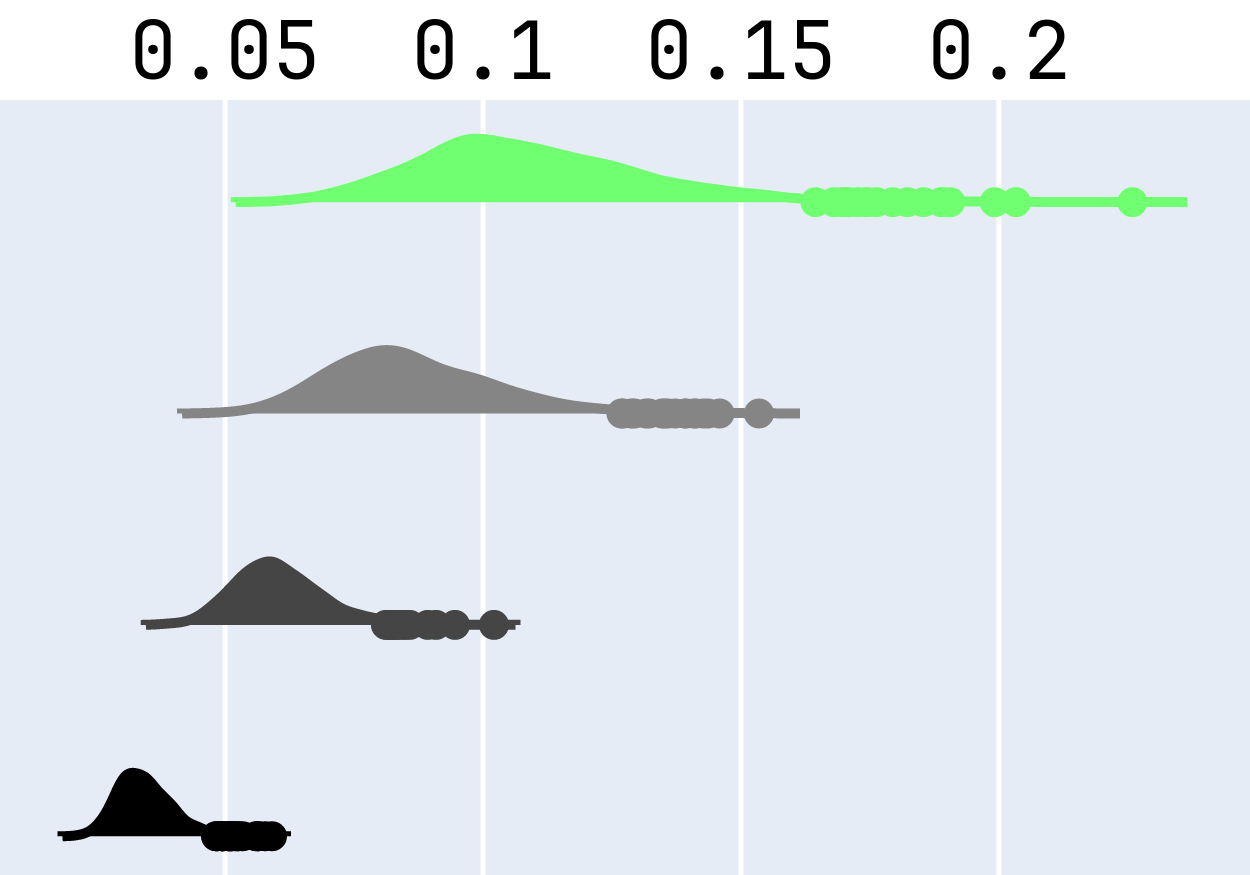
\includegraphics[width=\linewidth]{images/npsk_MSS_0.png}
      \end{minipage}
      \hspace{0.015\textwidth}%
      \begin{minipage}[t]{0.31\textwidth}
        \centering
        \normalsize\bfseries P-Loss\\[0.3em]
        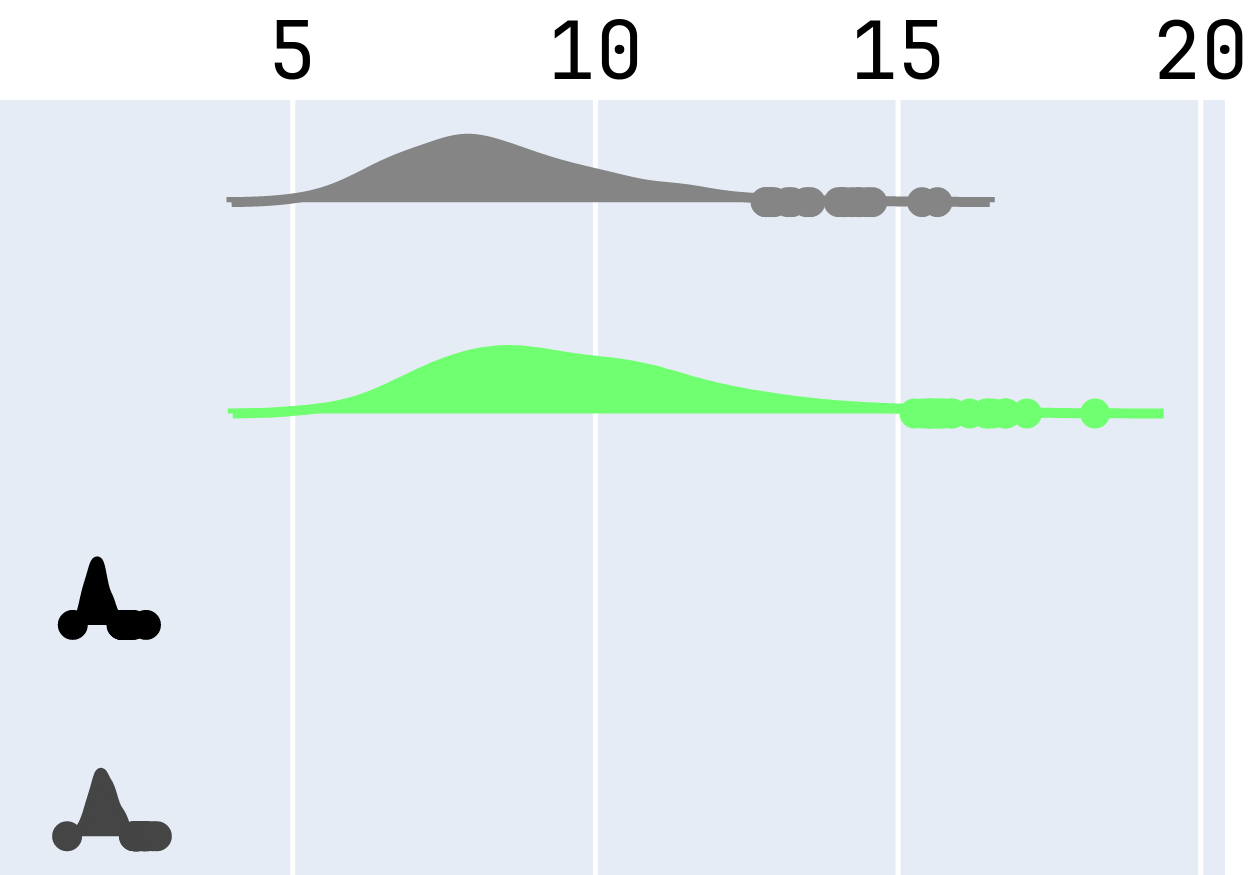
\includegraphics[width=\linewidth]{images/npsk_P-Loss_0.png}
      \end{minipage}
      \hspace{0.01\textwidth}%
      \begin{minipage}[t]{0.31\textwidth}
        \centering
        \normalsize\bfseries Likert\\[0.3em]
        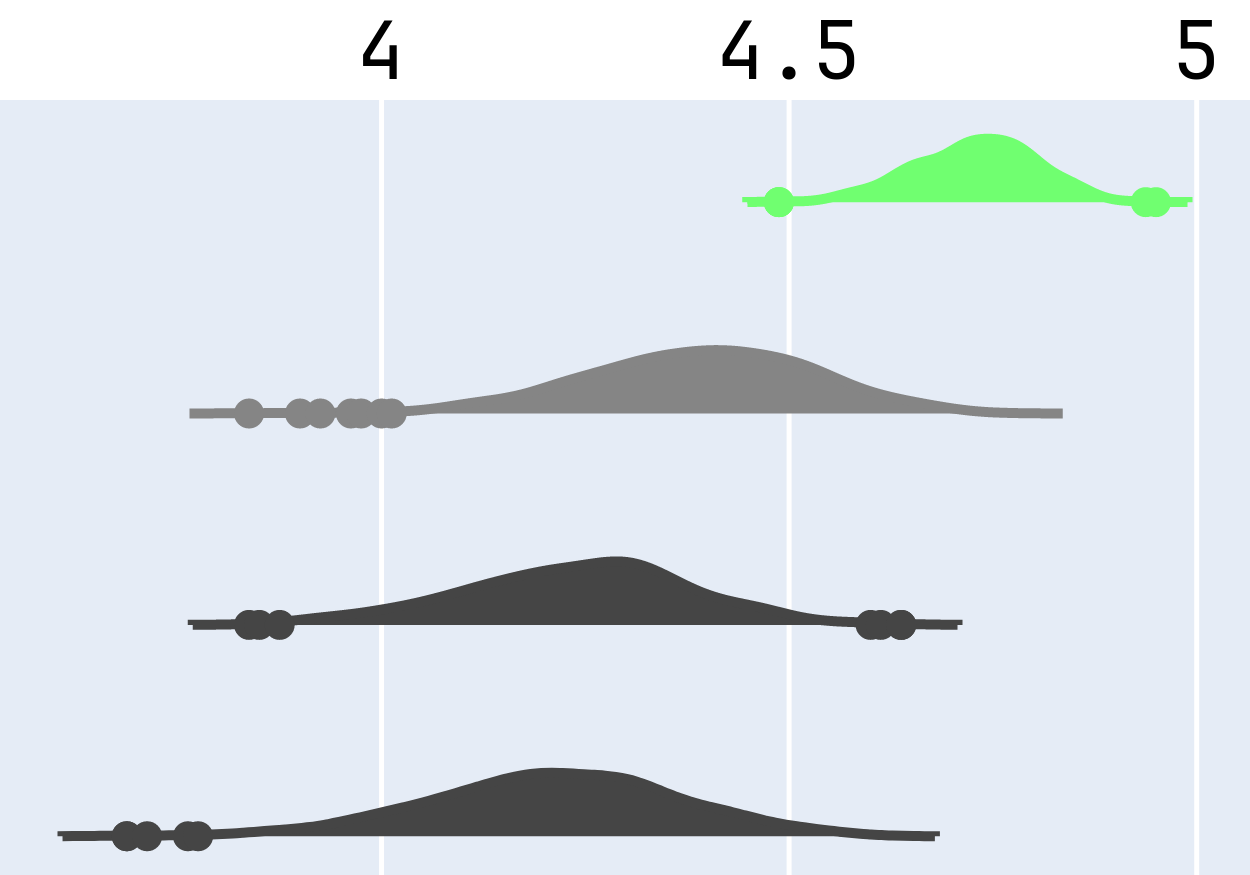
\includegraphics[width=\linewidth]{images/npsk_likert_0.png}
      \end{minipage}
    \end{minipage}
  \end{minipage}
  \label{fig:npsk_p0}
}\\[0.5em]

% 2nd row
\subfloat[\AddSineSaw~bootstrapped distributions and ranks given by NPSK.]{
  \begin{minipage}{\textwidth}
    \begin{minipage}{0.03\textwidth}
      \footnotesize\raggedleft
      \vspace{0.5cm}
      SIMSE\\[0.6cm]
      L1\\[0.65cm]
      JTFS\\[0.65cm]
      DTW
    \end{minipage}%
    \begin{minipage}{0.98\textwidth}\centering
      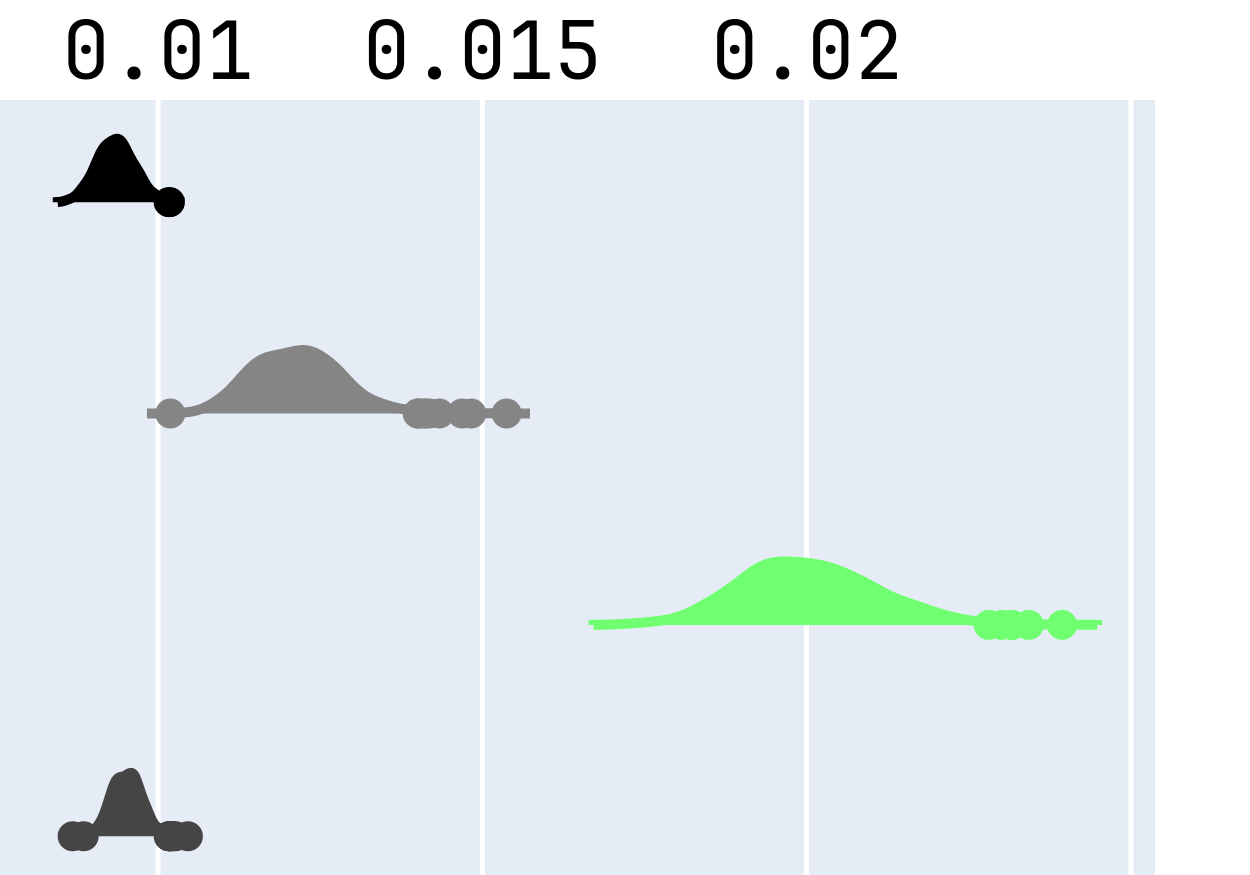
\includegraphics[width=0.31\textwidth]{images/npsk_MSS_1.png}%
      \hspace{0.015\textwidth}%
      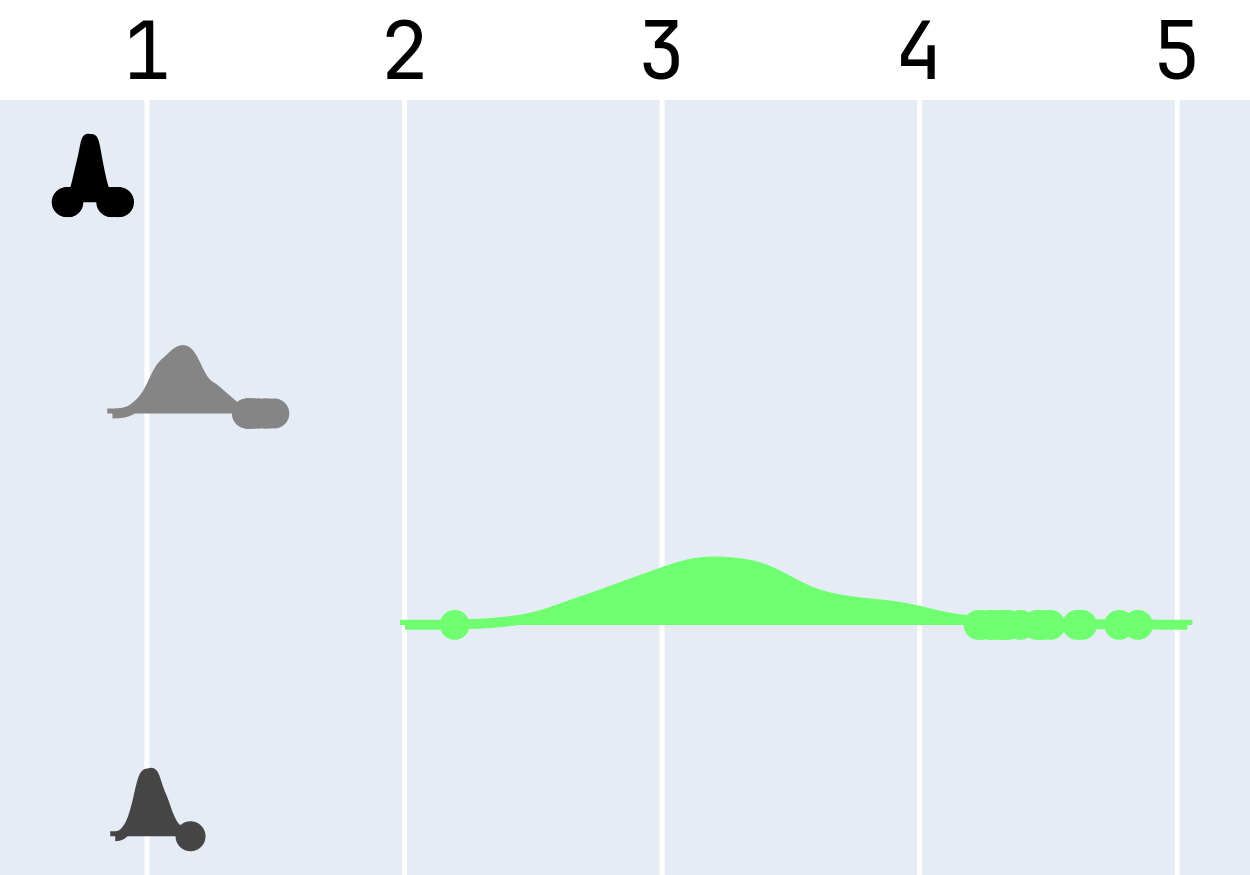
\includegraphics[width=0.31\textwidth]{images/npsk_P-Loss_1.png}%
      \hspace{0.015\textwidth}%
      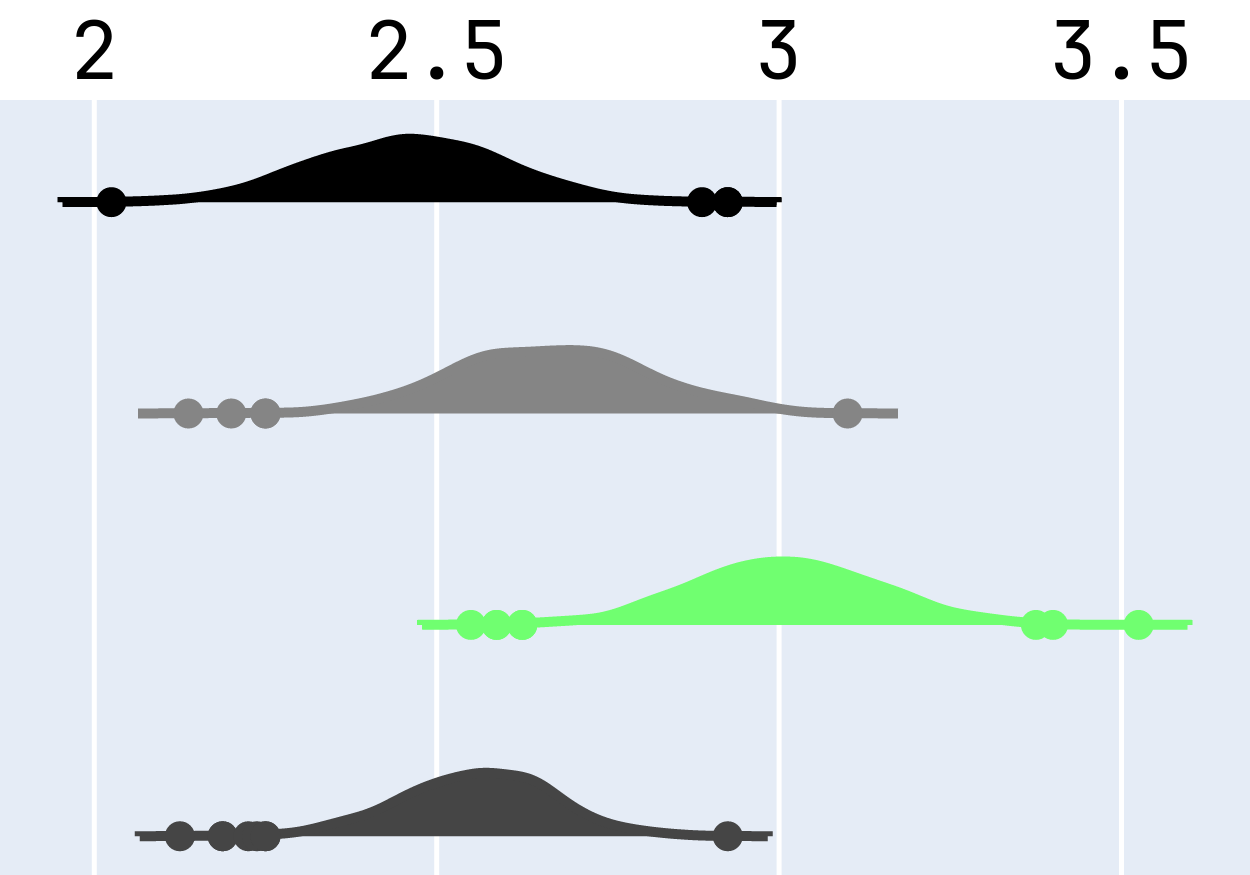
\includegraphics[width=0.31\textwidth]{images/npsk_likert_1.png}
    \end{minipage}
  \end{minipage}
  \label{fig:npsk_p1}
}\\[0.5em]

% 3rd row
\subfloat[\AmpMod~bootstrapped distributions and ranks given by NPSK.]{
  \begin{minipage}{\textwidth}
    \begin{minipage}{0.03\textwidth}
      \footnotesize\raggedleft
      \vspace{0.5cm}
      SIMSE\\[0.6cm]
      L1\\[0.65cm]
      JTFS\\[0.65cm]
      DTW
    \end{minipage}%
    \begin{minipage}{0.98\textwidth}\centering
      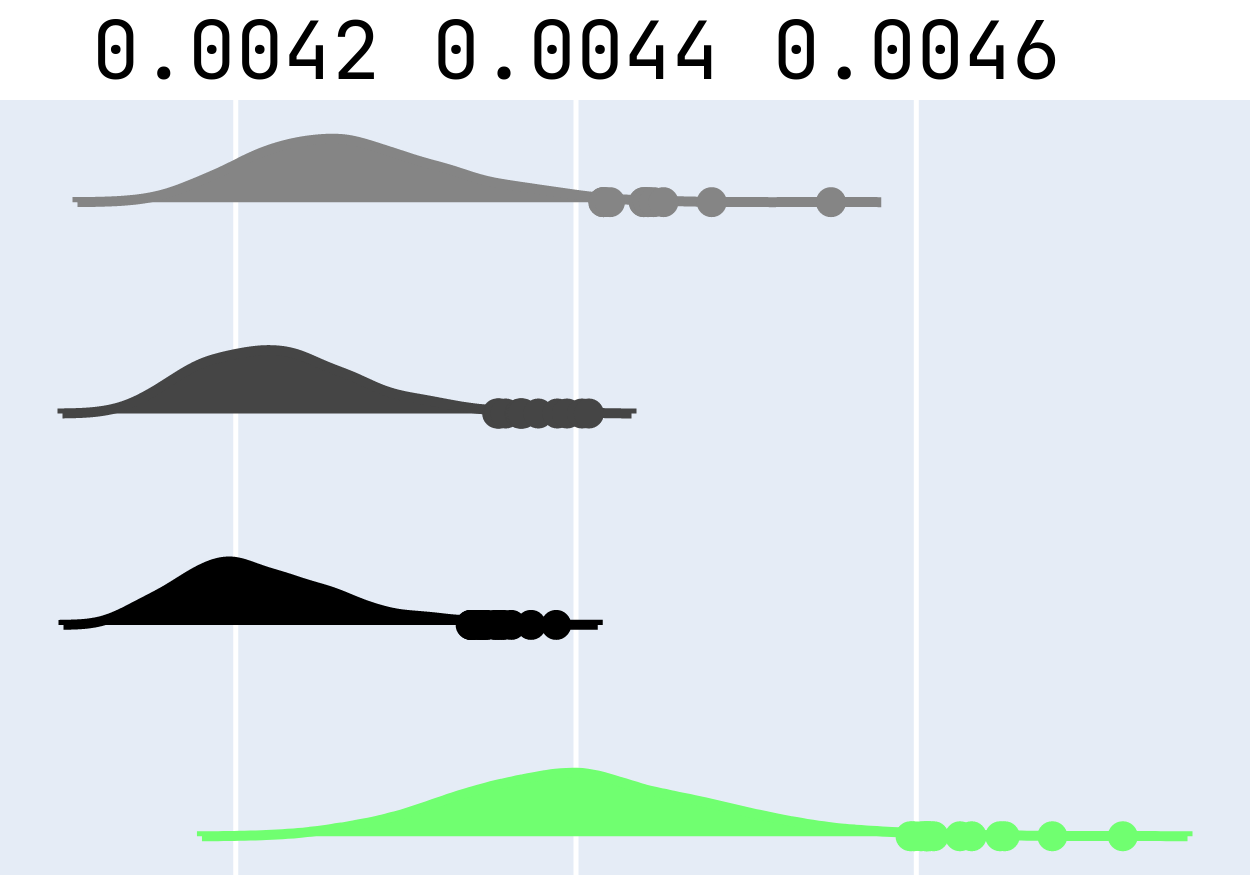
\includegraphics[width=0.31\textwidth]{images/npsk_MSS_2.png}%
      \hspace{0.015\textwidth}%
      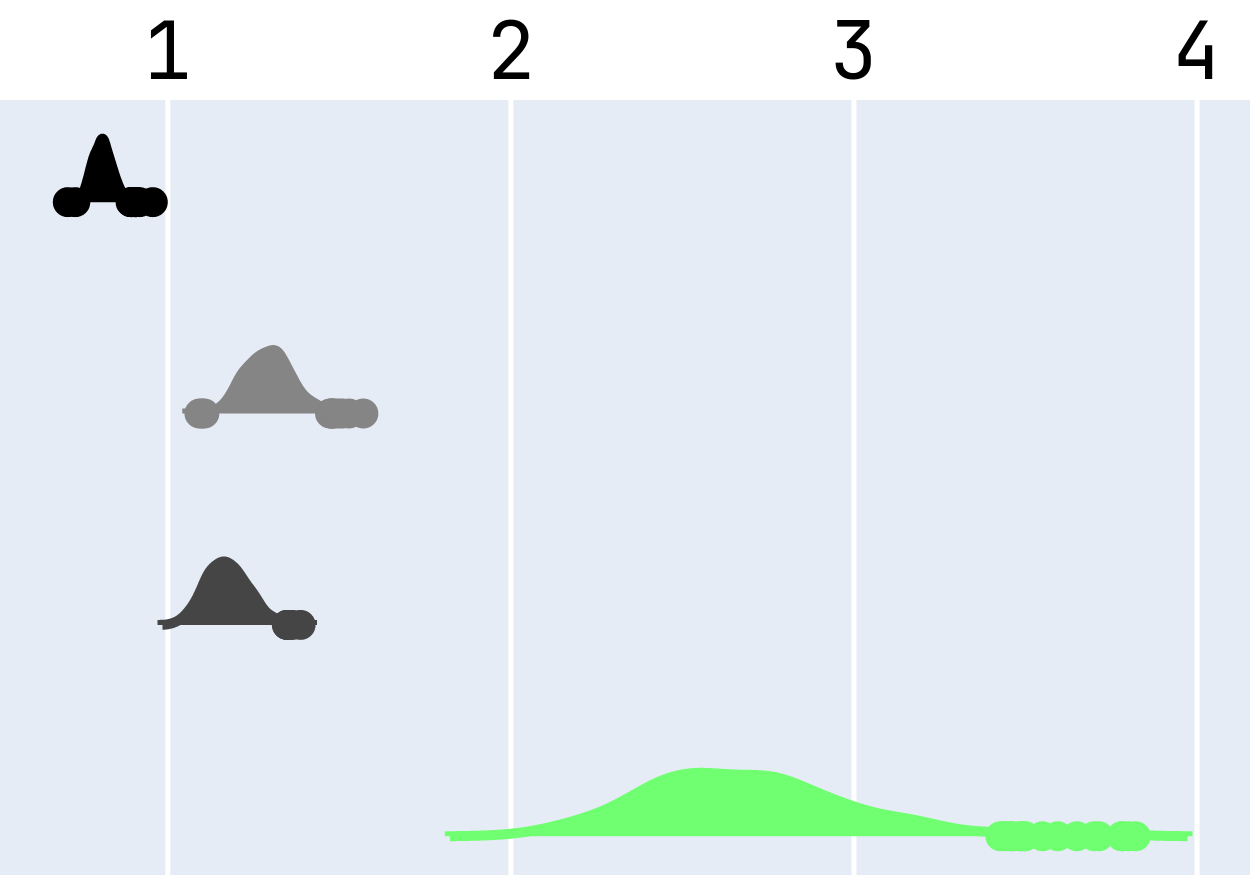
\includegraphics[width=0.31\textwidth]{images/npsk_P-Loss_2.png}%
      \hspace{0.015\textwidth}%
      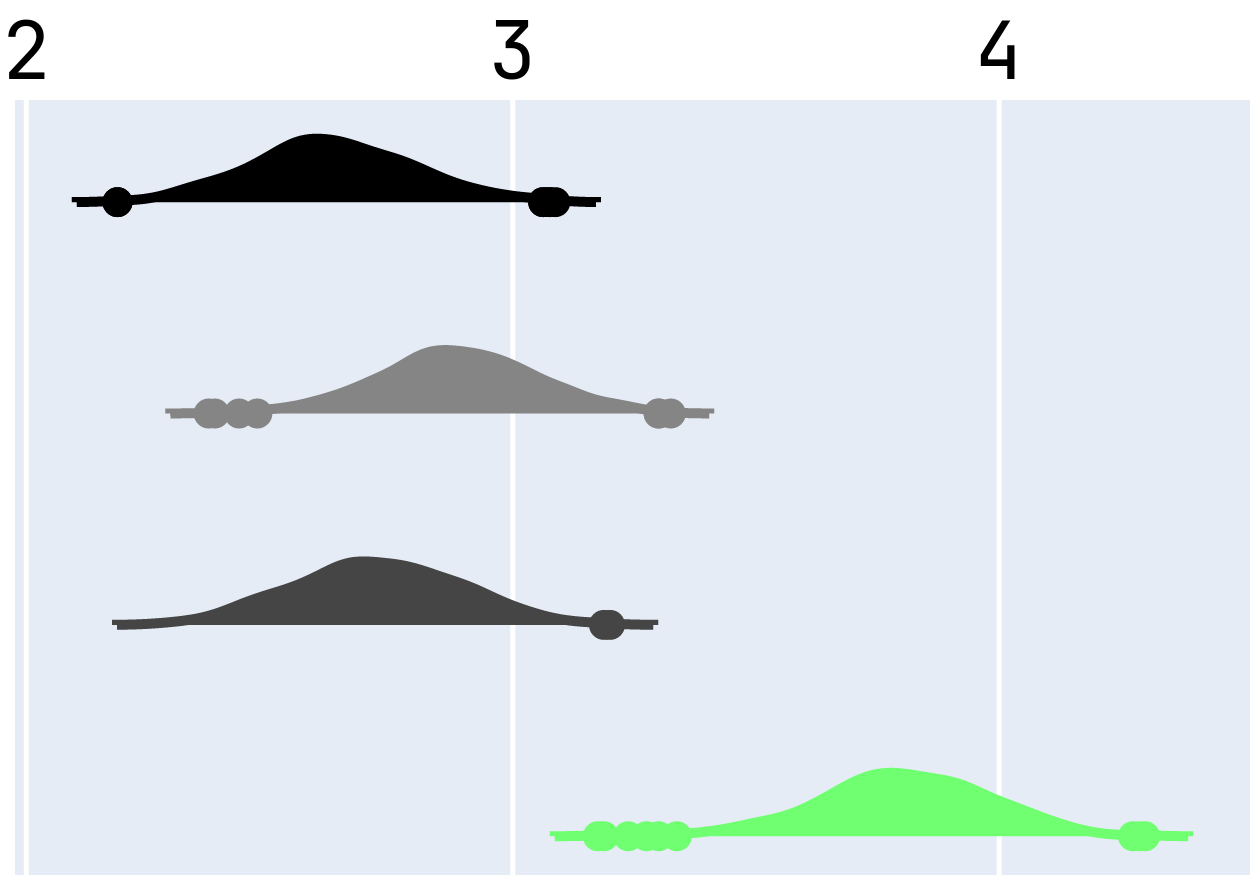
\includegraphics[width=0.31\textwidth]{images/npsk_likert_2.png}
    \end{minipage}
  \end{minipage}
  \label{fig:npsk_p2}
}\\[0.5em]

% 4th row
\subfloat[\FMMod~bootstrapped distributions and ranks given by NPSK.]{
  \begin{minipage}{\textwidth}
    \begin{minipage}{0.03\textwidth}
      \footnotesize\raggedleft
      \vspace{0.5cm}
      SIMSE\\[0.6cm]
      L1\\[0.65cm]
      JTFS\\[0.65cm]
      DTW
    \end{minipage}%
    \begin{minipage}{0.98\textwidth}\centering
      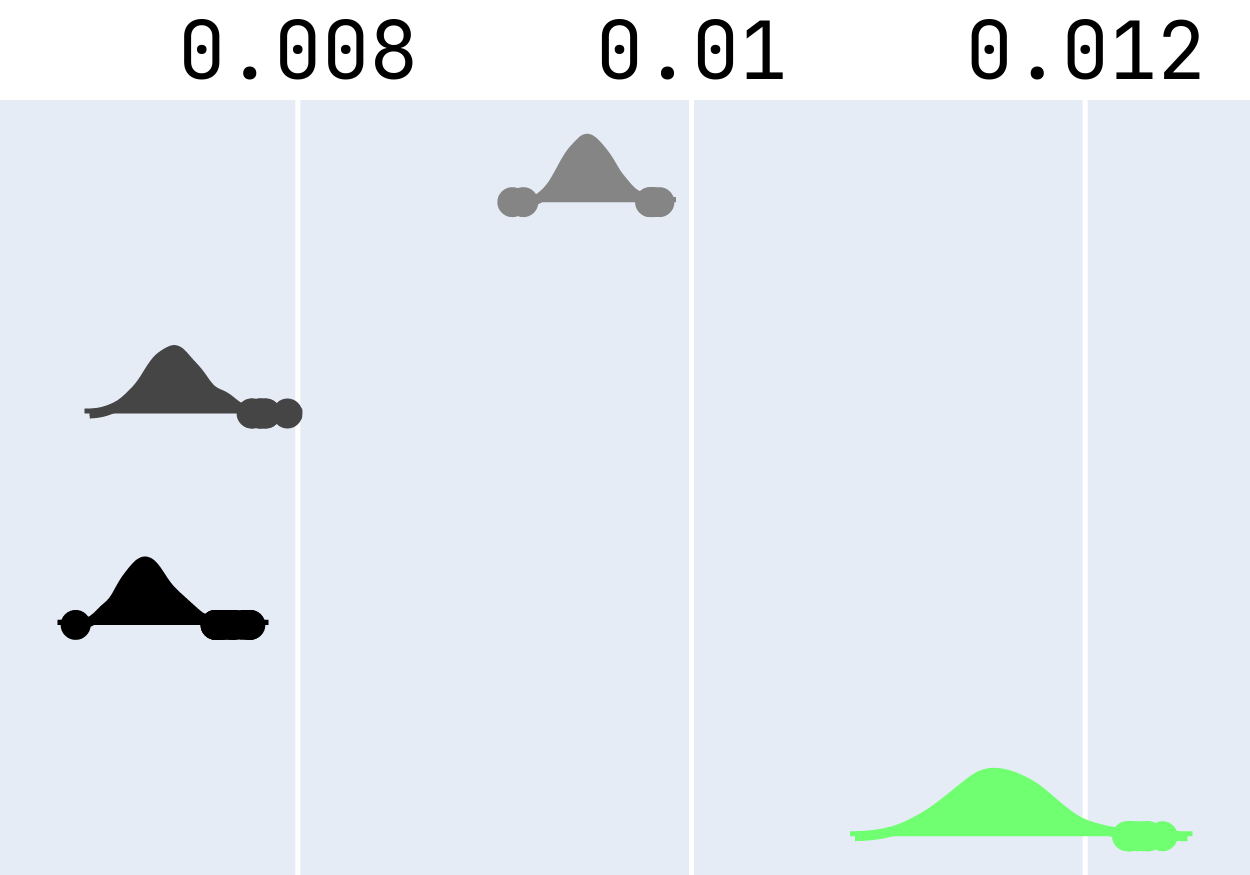
\includegraphics[width=0.31\textwidth]{images/npsk_MSS_3.png}%
      \hspace{0.015\textwidth}%
      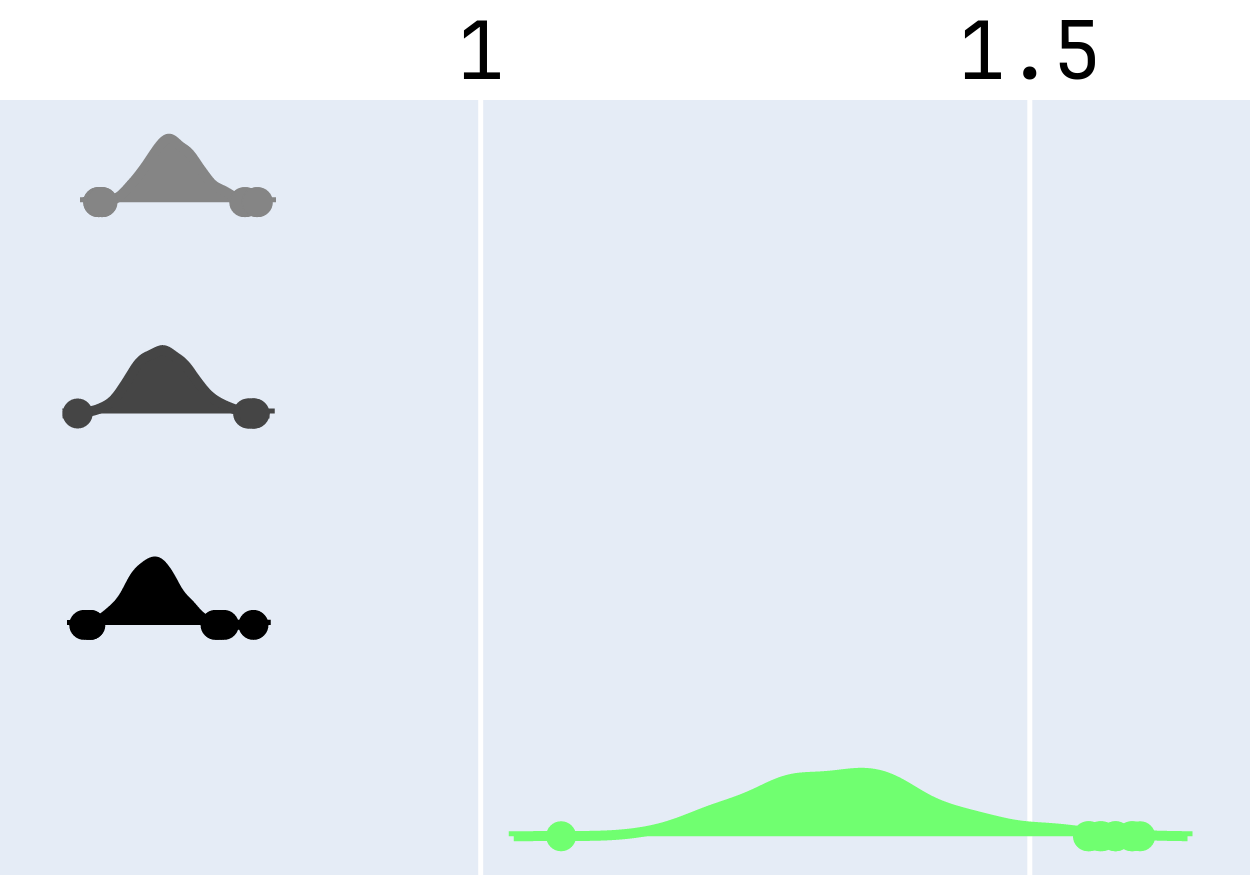
\includegraphics[width=0.31\textwidth]{images/npsk_P-Loss_3.png}%
      \hspace{0.015\textwidth}%
      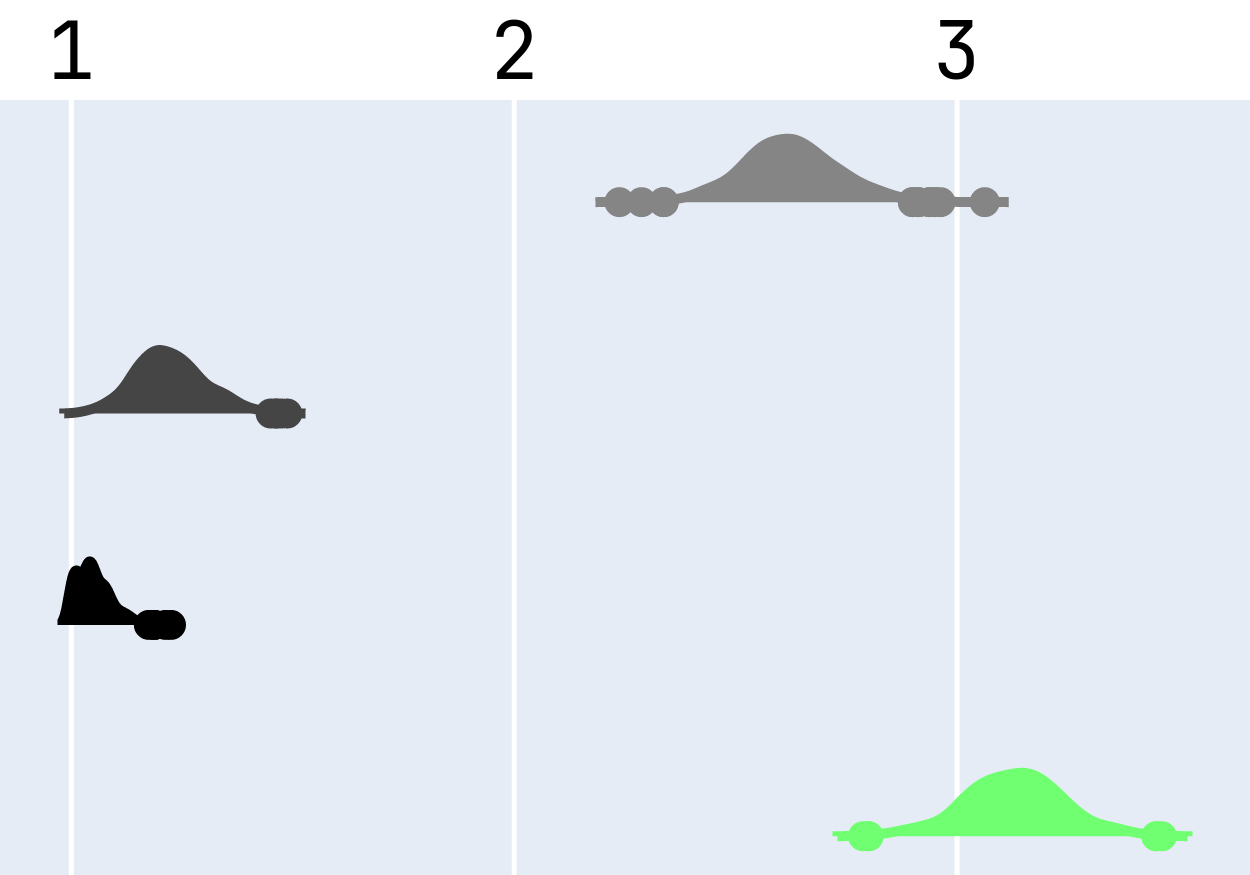
\includegraphics[width=0.31\textwidth]{images/npsk_likert_3.png}
    \end{minipage}
  \end{minipage}
  \label{fig:npsk_p3}
}

\caption{Distributions and ranks of the loss functions based on three different performance measures. From left to right, the performance measures are: MSS, P-Loss, and Likert. Higher values indicate better performance. Rank colors are \colorbox{rank1}{\textcolor{black}{\textbf{1}}} \colorbox{rank2}{\textcolor{white}{\textbf{2}}} \colorbox{rank3}{\textcolor{white}{\textbf{3}}} \colorbox{rank4}{\textcolor{white}{\textbf{4}}}.}
\label{fig:npsk_all}
\end{figure*}


\subsubsection{\BPNoise}
For this synthesizer program, the spectrogram-based models performed the best. This makes intuitive sense, as the visual effects of a band-pass filter on white noise are readily apparent in a spectrogram. As shown in Figure~\ref{fig:npsk_p0}, manual hearing test and MSS selected \SIMSESpec~as the best performer and \LoneSpec~as the second-best performer, while P-loss gave the reverse order. 


\subsubsection{\AddSineSaw}
As shown in Figure~\ref{fig:npsk_p1}, JTFS was the best performing loss function in all evaluation methods. Moreover, all evaluation methods produced identical results. 

\subsubsection{\AmpMod}
IP-Loss and manual hearing tests yield identical rankings, and MSS results vary for for ranks 2 to 4. It is not surprising that MSS results differ from the hearing tests, as we saw in Table~\ref{tab:kruskal_auto}, MSS showed no significant differences between groups. As shown in Figure~\ref{fig:npsk_p2}, all models selected \DTWEnv~as the best performer. This may be due to \DTWEnv's focus on periodic changes in loudness.

\subsubsection{\FMMod}
\DTWEnv~is again the best performer here. As shown in Figure~\ref{fig:npsk_p3}, all methods of analysis gave identical rankings to all programs.

\subsection{Consistency In Rankings}
\label{sec:consistency_in_rankings}
\subsubsection{Manual Ranks} Agreement between the manually assigned scores is measured using Spearman’s rank correlation, which provides both a correlation coefficient ($\rho$) ranging from –1 (perfect negative correlation) to 1 (perfect positive correlation), and a p-value testing the null hypothesis of no correlation~\cite{spearman1987proof,rebekic2015pearson}. Across all programs, the correlation was very strong ($\rho = 0.86$, $p < 10^{-180}$). Per-program correlations were also very strong: $\rho = 0.71$ for \BPNoise{} ($p < 10^{-25}$), $\rho = 0.64$ for \AddSineSaw{} ($p < 10^{-19}$), $\rho = 0.84$ for \AmpMod{} ($p < 10^{-43}$), and $\rho = 0.85$ for \FMMod{} ($p < 10^{-44}$). 

Table~\ref{tab:combined_ranks} shows the SNPK rankings of bootstrapped evaluation results for each program. Both MSS and P-Loss gave a different rank from the hearing results in 3 out of 16 cases, which shows consistency between automatic and manual hearing tests, at least for the simple programs used in this work. We also observe that top ranks were consistent across performance evaluation methodologies, with the exception of P-Loss in \BPNoise, which narrowly picks a different spectrogram-based loss function.
% \noindent\textit{Ranks that differ from the hearing test are marked with an asterisk.}

\begin{table}[htbp]
\centering
\begin{minipage}{0.45\textwidth}
    \centering
    \begin{tabular}{|c|c|c|c|}
    \hline
    \textbf{Function} & \textbf{MSS} & \textbf{P-LOSS} & \textbf{Hearing} \\
    \hline
    \textbf{SIMSE} & 1\phantom{*} & 2* & 1\phantom{*} \\
    \textbf{L1}    & 2\phantom{*} & 1* & 2\phantom{*} \\
    \textbf{JTFS}  & 3\phantom{*} & 4* & 3\phantom{*} \\
    \textbf{DTW}   & 4*           & 3\phantom{*} & 3\phantom{*} \\
    \hline
    \end{tabular}
    \caption{\footnotesize \BPNoise~ranks}
    \label{tab:p0}
\end{minipage}%
\hspace{1cm}
\begin{minipage}{0.45\textwidth}
    \centering
    \begin{tabular}{|c|c|c|c|}
    \hline
    \textbf{Function}& \textbf{MSS} & \textbf{P-LOSS} & \textbf{Hearing} \\
    \hline
    \textbf{SIMSE} & 4\phantom{*} & 4\phantom{*} & 4\phantom{*} \\
    \textbf{L1} & 2\phantom{*} & 2\phantom{*} & 2\phantom{*} \\
    \textbf{JTFS} & 1\phantom{*} & 1\phantom{*} & 1\phantom{*} \\
    \textbf{DTW} & 3\phantom{*} & 3\phantom{*} & 3\phantom{*} \\
    \hline
    \end{tabular}
    \caption{\footnotesize \AddSineSaw~ranks}
    \label{tab:p1}
\end{minipage}

\vspace{0.5cm} % Adds vertical space between rows of tables

\begin{minipage}{0.45\textwidth}
    \centering
    \begin{tabular}{|c|c|c|c|}
    \hline
    \textbf{Function} & \textbf{MSS} & \textbf{P-LOSS} & \textbf{Hearing} \\
    \hline
    \textbf{SIMSE} & 3* & 4\phantom{*} & 4\phantom{*} \\
    \textbf{L1}    & 2\phantom{*} & 2\phantom{*} & 2\phantom{*} \\
    \textbf{JTFS}  & 4* & 3\phantom{*} & 3\phantom{*} \\
    \textbf{DTW}   & 1\phantom{*} & 1\phantom{*} & 1\phantom{*} \\
    \hline
    \end{tabular}
    \caption{\footnotesize \AmpMod~ranks}
    \label{tab:p2}
\end{minipage}%
\hspace{1cm}
\begin{minipage}{0.45\textwidth}
    \centering
    \begin{tabular}{|c|c|c|c|}
    \hline
    \textbf{Function} & \textbf{MSS} & \textbf{P-LOSS} & \textbf{Hearing} \\
    \hline
   \textbf{SIMSE} & 2\phantom{*} & 2\phantom{*} & 2\phantom{*} \\
    \textbf{L1} & 3\phantom{*} & 3\phantom{*} & 3\phantom{*} \\
    \textbf{JTFS} & 4\phantom{*} & 4\phantom{*} & 4\phantom{*} \\
    \textbf{DTW} & 1\phantom{*} & 1\phantom{*} & 1\phantom{*} \\
    \hline
    \end{tabular}
    \caption{\footnotesize \FMMod~ranks}
    \label{tab:p3}
\end{minipage}
\end{table}





\subsection{Takeaways}
An important takeaway is that the loss function that yields the best sound-matching outcomes varies depending on the synthesizer program. This is perhaps due to the interaction between how the parameters of the synthesizer influence the sound, and the core sonic features of the loss function.

We also see that the \DTWEnv{} and \SIMSESpec{} (to our knowledge, not previously used in iterative sound-matching), lead to the best results in three of the four programs. This shows room for further creative approaches to differentiable sound-similarity measures, particularly since we observed that SOTA loss functions can be ineffective depending on the design of a synthesizer. 

Finally, we surprisingly see somewhat consistent results between the rankings assigned by manual hearing tests (which we take as the ground truth), and automatic measures of P-Loss and MSS. Due to the simplicity of our programs and the occasional deviations, we cannot conclude that these automatic measures are substitutes for human hearing tests.


\section{Summary, Weaknesses, and Conclusion}
\label{sec:summary_conclusion}
\textbf{Summary:} Sound-matching is an umbrella term for the algorithmic programming of audio synthesizers, often with the goal of assisting sound designers. Here we provided a history of sound-matching, major issues in the field, and discussed the importance of ``differentiable iterative sound-matching'' as a natural extension of current literature.

The main hypothesis tested here is whether the performance of differentiable loss functions is influenced by the synthesis techniques used for sound-matching. We created iterative sound-matching experiments by combining four different loss functions with four different sound synthesis programs. We ranked the performance of the iterative sound-matching pipelines for every loss function and program, and observed that the success of the pipeline (that is, how closely the output sound matches the target sound) is program dependent. In other words, different synthesizer programs work best with different loss functions. Notably, we see that our novel use of DTW and SIMSE based differentiable loss functions (\DTWEnv{} and \SIMSESpec) can outperform what are regarded as the SOTA loss functions in 3 of 4 cases, although this is highly synthesizer dependent. 

P-Loss and MSS have frequently been used as automatic performance measures, yet their ``preference'' has rarely been compared to human rankings. We observed that automatic performance measures and manual listening tests were often in agreement, despite this, manual verification of sound-matching results remains a necessity for future works.  

\textbf{Weaknesses:} 
While we cannot prove that a universally best similarity measure does not exist, we can advocate for more creativity in the field based on our findings. Compared to previous work, we presented a more cohesive approach to iterative sound-matching which utilizes a variety of loss functions and synthesis methods. However, there are many other methods of synthesis and sound-similarity that can be combined in practically infinite ways. Due to this large search space, we set arbitrary parameters for the various signal processing functions. We used bare-bones versions of STFT and JTFS with fixed parameters. We did not test complex synthesizers using parallel and sequential DSP functions. Arbitrary hyperparameters such as learning rate and max number of iterations were selected for the DL pipeline, and only the RMSProp optimizer was tested. 

 Like the majority of previous works, this work utilizes in-domain sounds; that is, the target sound is made by the synthesizer, and the parameters are already known. This simplifies the issues of measuring sound-similarity, but it is not a realistic scenario for practical sound-matching. This problem is left for future work, discussed in the next section.

\label{sec:future}
\textbf{Future Work: } The problem of periodic loss-landscapes, noted by many previous works, remains unaddressed~\cite{turian2020sorry,vahidi2023mesostructures,uzrad2024diffmoog,bruford2024synthesizer}. Perhaps this problem emerges due to the periodic nature of sound, which requires better loss landscape navigation methods. An optimizer that is more aware of fluctuations in the gradients would perhaps lead to better solutions than simple gradient descent. Viewing the sound-matching problem as ``the navigation of an agent from an arbitrary point in a gradient field to a target'' closely resembles many classical problems in the field of reinforcement learning (RL)~\cite{sutton2018reinforcement}. Naturally, the application of RL and other heuristic search techniques to the problem of iterative sound-matching would be an important contribution.

Contemporary works often involve the application of domain specific and computationally expensive loss functions~\cite{han2023perceptual,uzrad2024diffmoog}, use of large neural networks~\cite{hershey2017cnn,cramer2019look}, or complex ensemble methods~\cite{turian2022hear}. Such models are useful but intractable; furthermore, training them requires the definition of simpler loss functions, which emphasizes the need for further development of differentiable and expressive loss function implementations. 

Like nearly all previous work in sound-matching, the main measure of success here was the accurate \textit{replication} of sounds (or synth parameters) rather than imitation of sounds outside of the synthesizer's domain. Replication of arbitrary features of sounds is an important component of sound-design, though it is much harder to define or measure. Future works could explore loss functions which only measure certain characteristics of sound (such as \DTWEnv), and whether they can pave the way for better imitation sound-matching.

\bibliographystyle{IEEEtran}
\bibliography{references}
\end{document}


